% Введение
\section{Введение}
\vspace{0.5cm}

   В общей квантовой системе многих тел размерность гильбертова пространства растет экспоненциально с увеличением размера системы. Этот барьер мешает физикам извлекать информацию об этой квантовой системе. Для преодоления этой стены ученые пытаются использовать разные способы, одним из самых продуктивных является - QMC(Квантовый метод Монте-Карло). На сегодняшний день данную проблему нельзя решить путем прямой диагонализации гамильтониана из-за нехватки компьютерной мощности. Однако, методы машинного обучения весьма эффективны для извлечения данных из больших источников информации, в частности, их можно использовать для решения нашей проблемы. Если говорить формально то мы записываем нашу волновую функцию, зависящую от достаточного количества параметров, а затем настраиваем параметры, чтобы получить целевую волновую функцию. Искусственные нейронные сети среди множества алгоритмов МО прекрасно подходят для этой цели. В данной работе мы опробуем представление NQS(нейросетевое квантовое состояние), которое по своей сути является картой из конфигурационного пространства спинов в волновую функцию: мы настраиваем параметры сети таким образом, чтобы для каждой входной спиновой конфигурации выходное число было пропорционально амплитуде вероятности, и в совокупности с этим метод машинного обучения(ММO) для реконструкции основного состояния модели Изинга с поперечным полем(TFIM).




% Основные главы
\section{Теоретическая часть}
\subsection{Некоторые сведения из квантовой механики и статистической физики}
\vspace{0.5cm}
\begin{description}
  \item[Гильбертово пространство] - бесконечномерное линейное пространство, в котором определено понятие скалярного произведения, удовлетворяющее четырем аксиомам: аддитивности, однородности, симметрии и положительной определенности.
  \item[Волновая функция] (\( \psi \)) - комплекснозначная функция, используемая в квантовой механике для математического описания чистого квантового состояния изолированной квантовомеханической системы.
  \item[Гамильтониан] (\( \hat{H} \) или \( H \)) - оператор полной энергии системы.
  \item[Спин] - собственный момент импульса элементарных частиц.
  \item[Состояние] - это просто набор физических величин, которые описывают систему. Например, для движующегося в пространстве электрона это будут его координаты и импульс, а для кристаллической решетки - набор спинов атомов, находящихся в её узлах.
  \item[Квaнтовая запутанность] - это явление, когда группа частиц генерируется, взаимодействует или находится в пространственной близости таким образом, что квантовое состояние каждой частицы группы не может быть описано независимо от состояния остальных, в том числе когда частицы разделены большим расстоянием.
  \item[Модель Изинга] — математическая модель статистической физики, предназначенная для описания намагничивания материала.


\end{description}



\subsection{Искусственные нейронные сети}
\vspace{0.5cm}

\hspace{0.5cm} \textbf{Искусственная нейронная сеть} (далее - нейронная сеть) - это сложная дифференцируемая функция, задающая отображение из исходного признакового пространства в пространство ответов, все параметры которой могут настраиваться одновременно и взаимосвязанно (то есть сеть может обучаться end-to-end). В частном (и наиболее частом) случае представляет собой последовательность (дифференцируемых) параметрических преобразований.

\vspace{0.25cm}

\textbf{Теорема Цыбенко} (Универсальная теорема аппроксимации) - теорема, доказанная Джорджем Цыбенко в 1989 году, утверждает, что искусственная нейронная сеть прямой связи (англ. feed-forward; в которых связи не образуют циклов) с одним скрытым слоем может аппроксимировать любую непрерывную функцию многих переменных с любой точностью. Условиями являются: достаточное количество нейронов скрытого слоя, удачный подбор параметров.
\vspace{0.25cm}

Сложную функцию удобно представлять в виде суперпозиции простых, и нейронные сети обычно предстают перед программистом в виде конструктора, состоящего из более-менее простых блоков (слоёв, layers). Вот две простейшие их разновидности:
\vspace{0.25cm}
- \textbf{Линейный слой} (linear layer, dense layer) — линейное преобразование над входящими данными. Его обучаемые параметры — это матрица \( \mathbf{W} \) и вектор \( \mathbf{b} \): \( \mathbf{y} = \mathbf{Wx} + \mathbf{b} \). Такой слой преобразует \( n \)-мерные векторы в \( m \)-мерные.
\vspace{0.25cm}
- \textbf{Функция активации} (activation function) — нелинейное преобразование, поэлементно применяющееся к пришедшим на вход данным. Благодаря функциям активации нейронные сети способны порождать более информативные признаковые описания, преобразуя данные нелинейным образом. Может использоваться, например, ReLU (rectified linear unit), которая определяется как \( f(x) = \max(0, x) \), или сигмоида (\( \sigma \)), которая определяется как \( f(x) = \frac{1}{1 + e^{-x}} \). 

\vspace{0.25cm}
В качестве примера удобно будет рассмотреть модель логистической регрессии:

\vspace{0.25cm}
\textbf{Логистическая регрессия}(англ. logit model) — статистическая модель, применяется для прогнозирования вероятности возникновения некоторого события по значениям множества признаков. Эта регрессия выдаёт ответ в виде вероятности бинарного события (1 или 0).

Она применяется для прогнозирования вероятности возникновения некоторого события по значениям множества признаков. Нейронную сеть можно представить в виде вычислительного графа, где вершинам промежуточным соотвествуют преобразования. А каждое состояния между которыми происходят переход при преобразовании - \textbf {слои}. 

\begin{figure}[h]
    \centering
    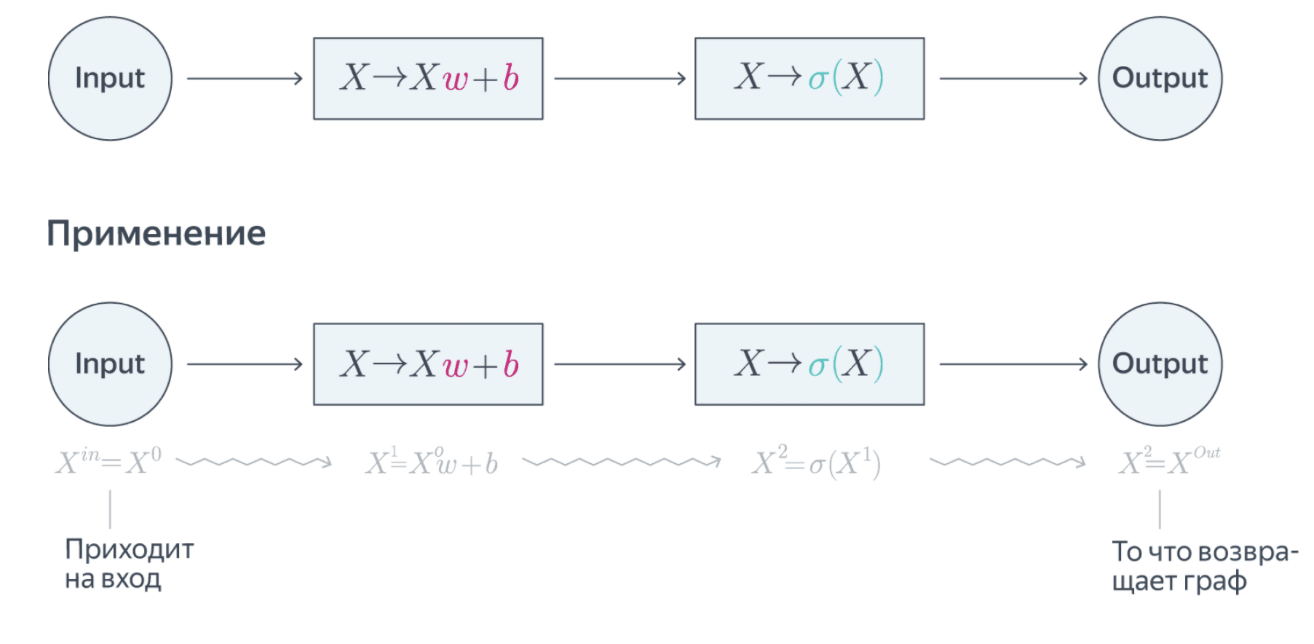
\includegraphics[width=0.8\linewidth]{Images/image1.png}

    \caption{Вычислительный граф для логистической регрессии}
    \label{fig:ваш_ярлык}
\end{figure}

Нейросеть, в которой есть только линейные слои и различные функции активации, называется \textbf{полносвязной (fully connected) нейронной сетью} или \textbf{многослойным перцептроном (multilayer perceptron, MLP)}.

Информация может течь по графу в двух направлениях. Применение нейронной сети к данным (вычисление выхода по заданному входу) часто называют \textbf{прямым проходом, или же forward propagation (forward pass)}.
 На этом этапе происходит преобразование исходного представления данных в целевое и последовательно строятся промежуточные (внутренние) представления данных — результаты применения слоёв к предыдущим представлениям. Именно поэтому проход называют прямым.

\begin{figure}[h]
    \centering
    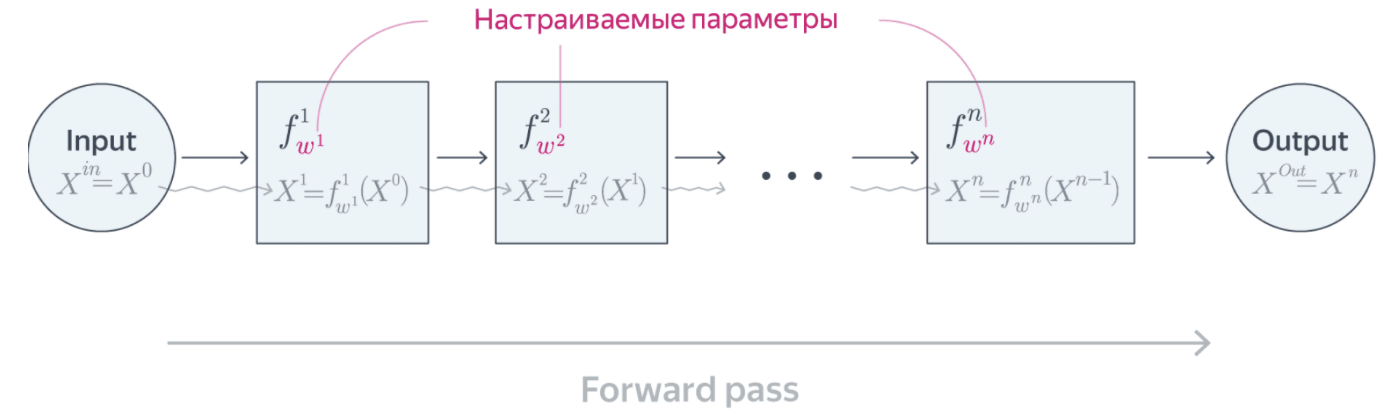
\includegraphics[width=0.8\linewidth]{Images/image2.png}

    \caption{Прямой проход}
    \label{fig:ваш_ярлык}
\end{figure}

При \textbf{обратном проходе}, или же \textbf{backward propagation (backward pass)}, информация движется от финального представления к исходному(так называемый механизм обратного распространения ошибки)

\begin{figure}[H]
    \centering
    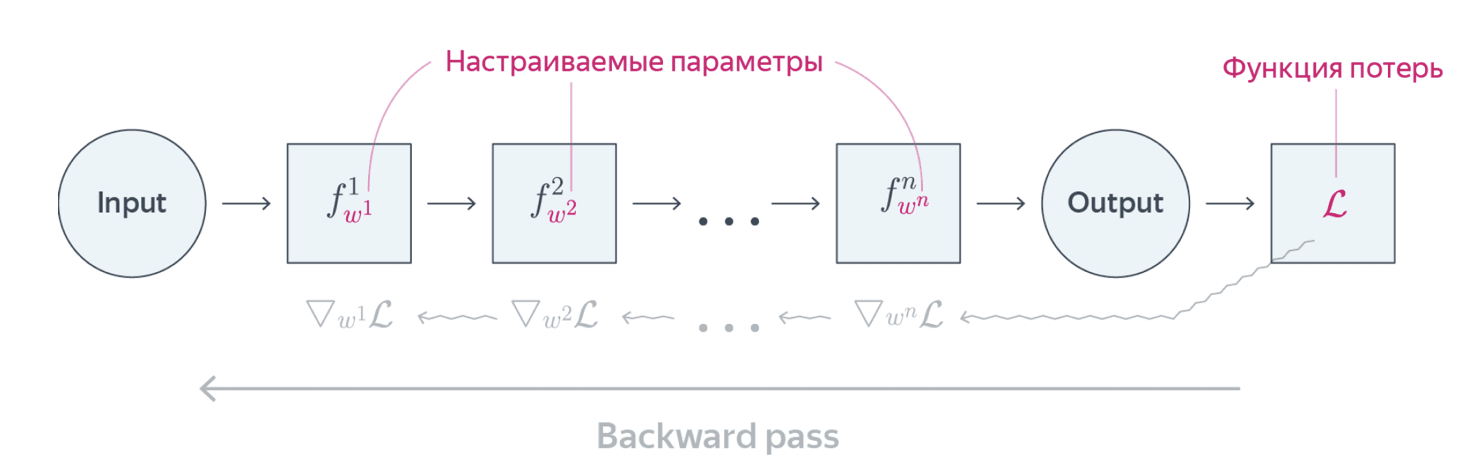
\includegraphics[width=0.8\linewidth]{Images/image3.png}
    \caption{Вычислительный граф для логистической регрессии}
    \label{fig:ваш_ярлык}
\end{figure}


\subsubsection{Ограниченная машина Больцмана(RBM) и модель поперечного поля Изинга(TFIM)}
\vspace{0.5cm}

Среди различных подходов, включающих контролируемое, неконтролируемое и повторное обучение, \textbf{ограниченные машины Больцмана (RBM)} выделяются как объекты, превосходно интерпретируемые в рамках устоявшейся статистической физики и теорий квантовой информации.
\vspace{0.5cm}

Сами машины Больцмана были созданы как способ представления распределения вероятностей P(v) путем определения ряда стохастических переменных(узлов) v и энергии взаимодействия между узлами E. Они расширяют  пространство физической системы, включая нефизические узлы и взаимодействия. Это скрытое или латентное пространство h может отражать корреляции более высокого порядка между видимыми узлами, значительно увеличивая выразительность сети, представляющей совместное распределение p(v,h). Чтобы облегчить практический алгоритм обучения параметров сети из данных, машины Больцмана стали ограниченными; то есть связи допускались только между видимыми и скрытыми узлами, но не внутри слоя (видимый-невидимый или скрытый-спрятанный). Таким образом, RBM сыграли исторически важную роль в генеративном предварительном обучении, уменьшении размерности, коллаборативной фильтрации, моделировании систем и многом другом. И сегодня RBM являются золотым стандартом в явных моделях плотности, где для оценки функции стоимости используется хорошо понятная стратегия Монте-Карло. 
\vspace{0.5cm}

Известно, что RBM является универсальным аппроксиматором. То есть при достаточном количестве скрытых единиц сеть способна приблизительно представить любое желаемое распределение вероятностей с произвольной точностью. Эта возможность сразу же поднимает перспективу использования RBM в качестве приближенных представлений волновых функций системы многих тел, называемых квантовыми состояниями нейронной сети. 
Теперь подробнее поговорим об RBM.
\vspace{0.5cm}

Она состоит из слоя видимых нейронов\( v_j \) и слоя скрытых нейронов \( h_i \), стохастических бинарных переменных, которые могут принимать значения 0 или 1. Параметры машины \( \lambda \) — это вес и смещение, которые определяют энергию \( U \) и параметризуют совместное распределение вероятностей \( p(v, h) \) в виде графической модели (см Рис.\ref{fig:rbm}). RBM может быть интерпретирована как волновая функция \(\Psi(v)\), где вероятность нахождения системы в состоянии \(v\) определяется квадратом модуля этой волновой функции: \(p(v) = |\Psi(v)|^2\), если обобщить её на комплексную фазу, где \( p(v) \) — это предельное распределение по видимым единицам \( p(v) = \sum_h p(v, h) \).
\vspace{0.5cm}

\textbf{Смещения.} Для видимой единицы \( v_j \) и скрытой единицы \( h_i \) соответствующие смещения в энергии RBM обозначаются как \( b_j \) и \( c_i \). Они действуют как локальное магнитное поле в энергии модели Изинга.

\textbf{Энергия.} По аналогии со статистической физикой энергия RBM определяется для совместной конфигурации \((v,h)\) видимых и скрытых единиц:
\[
U_\lambda(v,h) = - \sum_{i,j} W_{ij} h_i v_j - \sum_{j=1}^{V} a_j v_j - \sum_{i=1}^{H} b_i h_i
\]

\textbf{Генеративная модель.} Оформленная как задача неконтролируемого обучения, генеративная модель представляет собой статистическую модель распределения вероятностей, лежащего в основе некоторого набора данных.

\textbf{Скрытые единицы.} Во втором слое RBM находятся \( H \) единиц, обозначаемых вектором \( \mathbf{h} = (h_1, \ldots, h_H) \), представляющих латентные переменные и называемых 'скрытыми'. Количество скрытых единиц \( H \) может быть настроено для регулировки репрезентативной способности RBM.

\textbf{Совместное распределение.} RBM присваивает вероятность каждой совместной конфигурации \((\mathbf{v}, \mathbf{h})\) в соответствии с распределением Больцмана энергии:
\begin{equation}
p_{\lambda}(\mathbf{v}, \mathbf{h}) = \frac{1}{Z_{\lambda}} e^{-Г_{\lambda}}
\end{equation}

где \( Z_{\lambda} \) — нормирующая константа или статистическая сумма.

\textbf{Параметры.} Энергия RBM определяется через набор параметров нейронной сети \( \lambda = \{W, a, b\} \), состоящих из весов и смещений.

\textbf{Видимые единицы.} В первом слое RBM находятся \( V \) единиц, обозначенных вектором \( \mathbf{v} = (v_1, \ldots, v_V) \). Количество видимых единиц \( V \) фиксировано и соответствует количеству физических узлов или кубитов.

\textbf{Веса.} \( W_{ij} \) — это симметричное соединение или взаимодействие между видимой единицей \( v_j \) и скрытой единицей \( h_i \). Весы действуют как взаимодействие между переменными Изинга.

\begin{figure}[H]
    \centering
    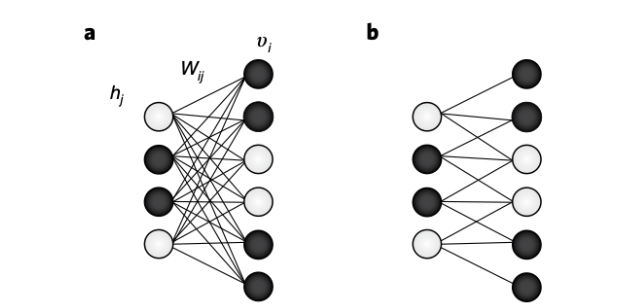
\includegraphics[width=0.8\linewidth]{Images/image4.png}
    \caption{\textbf{Ограниченная машина Больцмана.}}
    \label{fig:rbm}
\end{figure}

\begin{itemize}
    \item \textbf{a.} Стандартная, полностью связанная RBM, в которой все видимые единицы связаны с каждой скрытой единицей. Эта RBM способна кодировать волновую функцию с объемным законом запутывания.
    \item \textbf{b.} Разреженная RBM со связями между соседями. Такая машина вновь вводит идею пространственной локальности и способна представлять квантовые состояния со структурой запутывания по закону площади.
\end{itemize}

\vspace{0.5cm}

\subsubsection{Квантовая запутанность и кубит}


\textbf{Кубит} — наименьшая единица информации в квантовом компьютере (аналог бита в обычном компьютере), использующаяся для квантовых вычислений.\cite{qubitwiki}


    Как и бит, кубит допускает два собственных состояния, обозначаемых $\ket{0}$ и $\ket{1}$ (обозначения Дирака), но при этом может находиться и в их суперпозиции. В общем случае его волновая функция имеет вид $A\ket{0} + B\ket{1}$, где $A$ и $B$ называются амплитудами вероятностей и являются комплексными числами, удовлетворяющими условию $|A|^2 + |B|^2 = 1$. Состояние кубита удобно представлять как стрелку на сфере Блоха.
    
    При измерении состояния кубита можно получить лишь одно из его собственных состояний. Вероятности получить каждое из них равны соответственно $|A|^2$ и $|B|^2$. Как правило, при измерении состояние кубита необратимо разрушается, чего не происходит при измерении классического бита.
    

    Кубиты могут быть запутаны друг с другом. Квантовой запутанностью могут обладать два и более кубита, и она выражается в наличии особой корреляции между ними, которая невозможна в классических системах. Одним из наиболее простых примеров запутанности двух кубитов является состояние Белла $\ket{\Phi^+}$:
    
    \[
    \ket{\Phi^+} = \frac{1}{\sqrt{2}} (\ket{00} + \ket{11})
    \]

    Запись $\ket{00}$ обозначает состояние, когда оба кубита находятся в состоянии $\ket{0}$. Для состояния Белла характерно то, что при измерении первого кубита возможны два результата: 0 с вероятностью $\frac{1}{2}$ и конечным состоянием $\ket{\varphi'} = \ket{00}$, и 1 с вероятностью $\frac{1}{2}$ и конечным состоянием $\ket{\varphi''} = \ket{11}$. Как следствие, измерение второго кубита всегда даёт тот же результат, что и измерение первого кубита, т. е. данные измерений оказываются коррелированными.
\vspace{0,25cm}

\textbf{Закон площади}: Закон площади является одним из принципов, связывающих геометрическую структуру системы с ее квантовой запутанностью. Он утверждает, что количество запутанности между двумя подсистемами ограничено площадью поверхности, которая разделяет эти подсистемы. Это означает, что прирост запутанности между подсистемами пропорционален площади поверхности, а не объему пространства между ними. Закон площади имеет важное значение для понимания квантовых систем и может использоваться для анализа их свойств и динамики.
\vspace{0,25cm}

\textbf{PEPS (Projected Entangled Pair States): PEPS} - это класс квантовых состояний, используемых для представления квантовых многочастичных систем в теории тензорных сетей. Они представляют собой группу квантовых состояний, которые можно представить в виде тензорного произведения между конечным набором тензоров, каждый из которых описывает связи между некоторыми частицами в системе. PEPS предоставляют эффективный способ описания квантовых состояний с запутанностью, что позволяет анализировать их свойства и использовать их в квантовых вычислениях и других приложениях.
\vspace{0,25cm}

\textbf{Теория тензорных сетей (TN): Теория тензорных сетей} - это математический фреймворк, используемый для описания квантовых состояний многих частиц и анализа их свойств. В TN квантовые состояния представляются в виде тензорных произведений, в которых тензоры соединены друг с другом в определенной сетевой структуре. Эта сетевая структура позволяет эффективно описывать квантовые системы с большим количеством частиц и анализировать их запутанность, энергетические спектры и другие свойства. TN находят широкое применение в квантовых вычислениях, конденсированных средах и физике элементарных частиц.
\vspace{0,25cm}


Связь между ограниченными машинами Больцмана (RBM) и квантовыми запутанностями упрощается благодаря теоретическим рамкам, таким как область тензорных сетей (TN). Запутанность в TN определяется как индикатор эффективности представления волновой функции многих тел. Состояния, удовлетворяющие принципу области запутанности (принцип, утверждающий, что запутанность масштабируется пропорционально площади границы между подсистемами), успешно описываются тензорными сетями (TN), что означает, что число параметров, необходимых для их представления, полиномиально растет от числа кубитов. RBM могут быть непосредственно интерпретированы с точки зрения теории тензорных сетей, а их способность улавливать запутанность дает количественную оценку их выразительной способности, основанной на связности. Полная связность в обычных RBM ограничивает энтропию запутанности объёмом подсистемы, что может открыть возможность решения квантовых проблем многих тел, недоступных для TN.
\vspace{0,25cm}

Отсюда следует, что обычная RBM может быть способна эффективно кодировать волновые функции за пределами подмножества, определяемого PEPS. В некоторых случаях она способна делать это с очень небольшим количеством параметров (например, не зависящих от размера системы или полиномиально масштабирующихся с числом видимых единиц). Это может открыть возможность решения квантовых проблем многих тел, недоступных для TN, например, нахождения основных состояний систем с дальним взаимодействием (например, кулоновским или диполь-дипольным) или возбужденных состояний локальных гамильтонианов. В обоих случаях закон площади нарушается, и требуются представления, поддающиеся объемному закону запутывания. В других случаях, где может выполняться закон площади, включая проблему поиска основных состояний локальных гамильтонианов в трех измерениях, неизвестно, как эффективно скомпоновать тензоры представления TN. Однако здесь RBM могут работать так же хорошо, как и в более низких измерениях. 
Конечно, как и другие анзацы, RBM будут иметь различные преимущества и недостатки по сравнению с TN в зависимости от структуры волновой функции, на которую они нацелены. Действительно, между RBM и TN существуют четкие связи, которые помогают прояснить это соотношение и которые могут быть использованы для улучшения работы каждого из них. Например, некоторые классы PEPS могут быть записаны точно как RBM, и поэтому для этих состояний можно воспользоваться алгоритмами обучения, которые позволяют эффективно оптимизировать параметры даже в трех измерениях. 
В качестве альтернативы можно повысить эффективность машин Больцмана, еще больше ограничив межслойные связи короткими или разреженными, тем самым восстановив закон области, подходящий для изучения волновых функций основного состояния локальных гамильтонианов.
Естественной стратегией выхода за рамки парадигмы RBM является рассмотрение их глубоких обобщений. Теоретически известно, что они могут эффективно представлять любое квантовое состояние, возникающее в результате физической эволюции, но в данной работе мы будем рассматривать только RBM и её разреженную версию.
\vspace{0,25cm}

\subsubsection{Модель Изинга(TFIM) и нейросетевого квантого состояния(NQS)}


Как было оговорено ранее для описания квантовой системы со спином \(\frac{1}{2}\), используется нейронная сеть, которая имеет: видимый слой \(v = (v_1, v_2, \ldots, v_N)\), соответствующий реальной системе, и скрытый слой \(h = (h_1, h_2, \ldots, h_M)\), соответствующий вспомогательной структуре. Соединительные линии между видимыми узлами и скрытыми узлами представляют взаимодействия между ними, но внутри видимого слоя и скрытого слоя соединительных линий нет. Это и есть машина Больцмана(она же RBM). 
Вот более наглядная схема:



Волновую функцию системы многих тел можно рассматривать как отображение из пространства конфигураций спинов решетки в поле комплексных чисел. Явно это можно записать как
\[
\Psi(v, \lambda) = \sum_{\{h_j\}} \exp \left[ \sum_{i} a_i v_i + \sum_{j} b_j h_j + \sum_{i,j} w_{ij} v_i h_j \right]
\]

где \(v = \{v_i\}\) обозначает конфигурацию спинов, а \(\lambda = \{a, b, w\}\) — параметры весов нейронной сети. Настройка \(\lambda\) эквивалентна обучению нейронной сети. \(h_i = \{1, -1\}\) — скрытые переменные. Так как нет взаимодействий внутри видимого слоя и скрытого слоя, суммирование по спинам скрытых слоёв может быть просуммировано. Таким образом, волновая функция может быть записана проще:

\[
\Psi(v, \lambda) = e^{\sum_i a_i v_i} \prod_{j=1}^{M} 2 \cosh \left[ b_j + \sum_i w_{ij} v_i \right].
\]

Математически, это представление нейронной квантовой состояния (NQS) можно проследить до работы А. Колмогорова и В. Арнольда \cite{kolmogorov1957, arnold1963}. Это теорема Колмогорова-Арнольда о представлении, которая делает возможным выражение сложных функций высокой размерности как суперпозиции функций низкой размерности \cite{kolmogorov1936}.
\vspace{0,25cm}

\textbf{Модель Изинга с поперечным полем} — это квантовая версия классической модели Изинга. Она представляет собой решетку с взаимодействием ближайших соседей, определяемым выравниванием или невыравниванием проекций спинов вдоль оси \(z\), а также внешним магнитным полем, перпендикулярным оси \(z\) (без потери общности, вдоль оси \(x\)), которое создает энергетический перекос в пользу одного направления спина по оси \(x\) по сравнению с другим.

Важной особенностью этой модели является то, что, в квантовом смысле, проекция спина вдоль оси \(x\) и спиновая проекция вдоль оси \(z\) не являются взаимозаменяемыми наблюдаемыми величинами. То есть, они не могут наблюдаться одновременно. Это означает, что классическая статистическая механика не может описать эту модель, и требуется квантовая обработка.

В этой работе я фокусируюсь на ней, её гамильтониан имеет следующий вид:

\[
\mathcal{H} = -J \sum_{\langle i,j \rangle} \sigma^z_i \sigma^z_j - h \sum_{i} \sigma^x_i,
\]

где \(J\) и \(h\) являются параметрами межспинового взаимодействия и усилением внешнего поля соответственно. Матрицы Паули, \(\sigma_z\) и \(\sigma_x\), определяются как:

\[
\sigma_z = \begin{pmatrix}
1 & 0 \\
0 & -1
\end{pmatrix}, \quad \sigma_x = \begin{pmatrix}
0 & 1 \\
1 & 0
\end{pmatrix}.
\]

Эти матрицы используются для описания проекций спинов вдоль соответствующих осей.



\subsubsection{Нахождение параметров RBM по гамильтониану}

    Установив, что RBM's и их естественные расширения используются в качестве приближенных представлений квантовых состояний, возникает вопрос как найти оптимальные параметры (веса и смещения), чтобы стохастическая нейронная сеть наилучшим образом представляла целевую волновую функцию? Сначала мы рассмотрим определение целевой волновой функции как собственного вектора основного состояния некоторого гамильтониана, представляющего интерес. Это обычная задача в теоретической физике конденсированного вещества, атомной и молекулярной оптике, квантовой химии и входит в компетенцию обычных численных методов, основанных на вариационном принципе, таких как вариационный Монте-Карло.
    
    Нахождение основного состояния для заданного гамильтониана ($H$) можно представить как высокоразмерную задачу минимизации энергетического ожидания $\lambda$, кодирующего волновую функцию $\Psi$. По аналогии с приложениями машинного обучения, функция энергии $U$ является сильно нелинейной функцией потерь, значение и градиент которой оцениваются стохастически. В стандартных вариацонных расчетах Монте-Карло для оптимизации вариационных параметров волновой функции RBM используется такой современный метод, как стохастическая реконфигурация, о котором мы скоро поговорим.

    
    \begin{figure}[H]
        \centering
        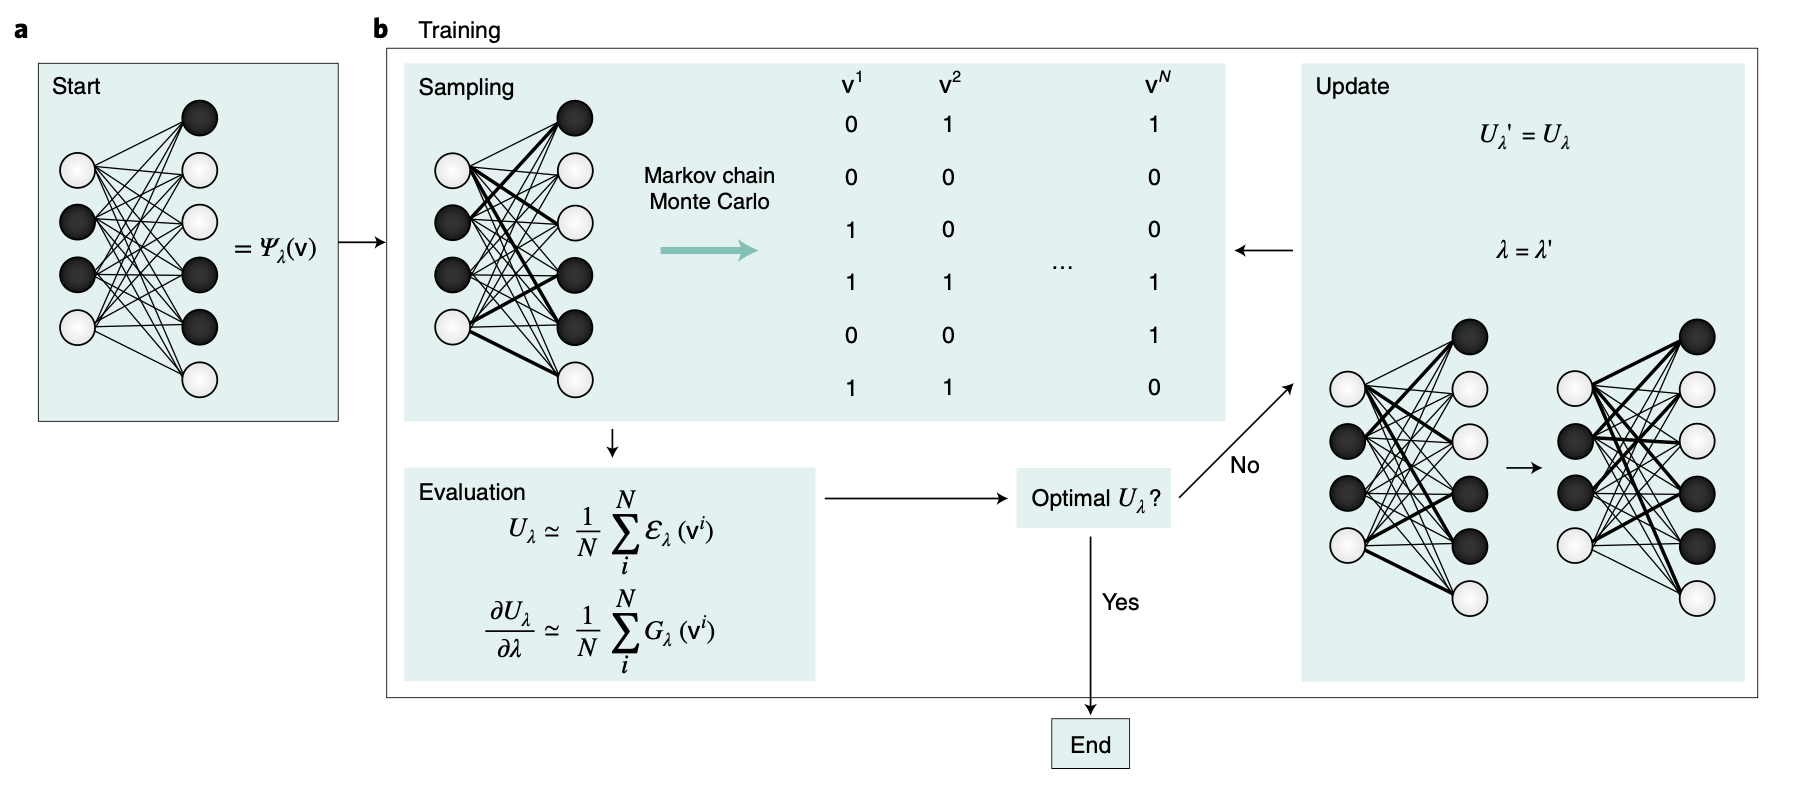
\includegraphics[width=0.9\linewidth]{Images/image6.png}
        \caption{\textbf{Использование вариационных методов для обучения параметров RBM.}}
        \label{fig:ваш_ярлык}
    \end{figure}
    
    \textbf{а}. RBM с комплексными весами используется для представления целевого многочастичного состояния в заданном вычислительном базисе $\langle v \mid \Psi \rangle$. Цель состоит в том, чтобы найти параметры RBM таким образом, чтобы функционал энергии \[
    U_{\lambda} = \frac{{\langle \Psi_{\lambda} \mid H \mid \Psi_{\lambda} \rangle}}{{\langle \Psi_{\lambda} \mid \Psi_{\lambda}\rangle}}
    \] достигал минимума. 
    
    \textbf{b}. На каждом шаге обучения генерируется большое количество \(N\) выборок \(v_1, v_2, \ldots, v_N\) в соответствии с вероятностным распределением, определяемым \(|\Psi_\lambda(v)|^2\), с использованием метода Монте-Карло на основе цепей Маркова. Эти выборки используются для оценки ожидаемого значения энергетического функционала \(\epsilon_\lambda(v) = \frac{\langle v | H | \Psi_\lambda \rangle}{\langle v | \Psi_\lambda \rangle}\) и его градиента \(G_\lambda(v)\). Существует много различных способов определения \(G_\lambda(v)\). Одним из эффективных способов может быть традиционный стохастический градиентный спуск, но также могут использоваться и другие улучшенные оценочные значения, например, стохастическая реконфигурация, о которой мы поговорим более подробно позже. Информация о градиенте используется для обновления параметров сети в направлении, уменьшающем энергетический функционал. Новые параметры снова используются, и процесс продолжается до тех пор, пока не будет найдена оптимальная энергия и обучение не завершится.
    \vspace{0,25cm}


    
    Помимо статического случая, важным расширением RBM-состояний является разрешение временной зависимости параметров сетки.
    В этом случае можно использовать зависящий от времени вариационный принцип Дирака и Френкеля для нахождения наилучшего вариационного состояния, решающего зависящее от времени уравнение Шредингера. Сложность в том, что решения уравнения Шрёдингера требует знания многочастичной волновой функции в многомерном гильбертовом пространстве, размер которой, как правило, растёт экспоненциально при увеличении числа частиц.
    
    Квантовые методы Монте-Карло открывает путь к непосредственному изучению многочастичных задач и многочастичных волновых функций без этих ограничений. Наиболее совершенные квантовые методы Монте-Карло дают точные решения многочастичных задачи системы бозонов без фрустраций, одновременно с приближенным, но как правило корректным описанием систем фермионов со взаимодействием. Большинство методов предназначены для нахождения волновой функции основного состояния системы, за исключением методов Монте-Карло для интегралов по траекториям и метода Монте-Карло для конечных температур, которые используются для вычисления матрицы плотности. Кроме стационарных задач можно решать также зависящее от времени уравнение Шрёдингера, хотя лишь приближено, ограничивая функциональную форму зависимой от времени волновой функции. Для этого разработан зависящий от времени вариационный метод Монте-Карло. 
    
    Полученные к настоящему времени результаты обнадеживают и в некоторых случаях улучшают существующие современные методы, например, были получены высокоточные волновые функции основного состояния для одномерных моделей. На примере этих моделей и будет происходить анализ параметров системы. 
    
    Несмотря на то, что вариационные приложения для системы многих тел на основе RBM наследуют все мощные идеи искусственных нейронных сетей и методов машинного обучения, они также унаследовали их основные недостатки. В частности, остается нерешенной задача определения того, какие сетевые архитектуры в наибольшей степени поддаются эффективному обучению и оптимизации. 

\subsection{Метод стохастической реконфигурации}
    \vspace{0.5cm}
    
    Метод SR (Steepest-Descent-Restricted) используется как метод оптимизации для нахождения целевых функций из некоторого общего набора пробных функций. Его можно рассматривать как вариацию метода крутого спуска (SD). 
    
    Квантовое состояние нашей системы является функцией от набора параметров нейронной сети $\{W_k\} \equiv \{a_i, b_j, w_{ij}\}$. Мы начнем с пробной функции $\Psi_T$, которая контролируется начальными параметрами $\{W_{k0}\}$. Рассмотрим небольшое изменение параметров $W_k = W_{k0} + \delta W_k$. При первом приближении новая волновая функция становится
    \[
        \Psi_T'(W) = \Psi_T(W) \left(1 + \sum_{k} \delta W_k \frac{\partial}{\partial W_k} \ln \Psi_T(W) \right).
    \]
    
    Введем локальный оператор $O_k$, такой что
    \[
    O_k = \frac{\partial \ln \Psi_T}{\partial W_k},
    \]
    и установим оператор идентичности $O_0 = 1$, тогда $\Psi_T$ может быть переписана в более компактной форме:
    \[
        \Psi_T'(W) = \sum_{k} \delta W_k O_k \Psi_T.
    \]
    Наша цель - найти волновую функцию основного состояния, такую что ожидаемое значение энергии ($U$) минимизируется. Очевидно, что $U$ зависит от параметров, вовлеченных в нейронную сеть. Процедура поиска основного состояния эквивалентна настройке параметров сети. Ключевой вопрос - стратегия обновления параметров от $W_0$ к $W$. Этот процесс подобен движению от начальной точки к целевой точке (основному энергетическому состоянию в нашем вопросе) в параметрическом пространстве. Параметрический путь, соединяющий начальную точку с целевой, определяется "принципом наименьшего действия" в параметрическом пространстве, как будет показано ниже.
    
    В методе SR параметры обновляются стратегиями
    \begin{equation} \label{eq:wi}
        w_i \rightarrow w_i + \Delta t \cdot \sum_k  s_{ik}^{-1} f_k
    \end{equation}
    где $s_{ik}$ - это метрика параметрического пространства, которая будет ясна из последующего обсуждения. Наша задача здесь - показать, что эта стратегия является требованием принципа наименьшего действия. Для этого мы сначала вводим обобщенные силы
    \[
    f_k = -\frac{\partial U}{\partial w_k}
    \]
    

    Тогда изменения энергии $U$, связанные с изменением $w$, можно записать как
    \[
    \Delta U = \frac{dU}{dw_i} \ dw_i = \frac{dU}{dw_i} dt \cdot s_{ik}^{-1} f_k = - dt \cdot s_{ik}^{-1} \frac{dU}{dw_i} \frac{dU}{dw_k}.
    \]
    Теперь, если мы определим $s_{ik} \Delta W_i \Delta W_k = \Delta s$ как линейный элемент в пространстве параметров, то
    \[
    \Delta s = -{\Delta U}{\Delta t}.
    \]
    
    В форме интегрирования это не что иное, как
    \[
    \int ds = S = \int dt \mathcal{L},
    \]
    где $S$ - "действие" итерационного процесса при поиске основного состояния системы, а $\mathcal{L}$ - его соответствующий "лагранжиан". Форма траектории в пространстве параметров при обновлении параметров определяется соответствующим принципом наименьшего действия. Это физический смысл метода SD. Метод SD является частным случаем метода SR, метрика пространства параметров которого является простой декартовой метрикой
    \[
    \Delta s = \sum_k |w_k' - w_k|^2
    \]
    Однако в общем случае у нас нет оснований считать пространство параметров таким простым. Поэтому мы должны ввести метрику так, чтобы
    \[
    \Delta s = \sum_{i,j} s_{ij}(w_i' - w_i)(w_j' - w_j)
    \]
    Именно по этой причине в уравнении (\ref{eq:wi}) появляется $s_{ik}$.
    Очевидно, что определение $s_{ik}$ является ключом к вопросу. На этот счет метод SR говорит нам, что
    \begin{equation} \label{eq:sik}
    s_{ik} = \langle O_i O_k \rangle - \langle O_i \rangle \langle O_k \rangle.
    \end{equation}
    С точки зрения информационной геометрии это очень естественно. Рассмотрим общее распределение данных $p(x; \theta)$, информационную матрицу Фишера или риманову матрицу, определяемую как
    \[
    g_{ik} = \int p(x; \theta) \frac{\partial \ln p(x; \theta)}{\partial \theta_i} \frac{\partial \ln p(x; \theta)}{\partial \theta_k} \, dx = \langle \partial_i \ln p \partial_k \ln p \rangle 
    \]
    В нашем квантовом состоянии нейронной сети вероятность считается (наша волновая функция ограничена вещественными полями)
    \[
    p(s, w_k) = \frac{|\Psi(s, w_k)|^2}{\langle \Psi | \Psi \rangle} = \frac{\Psi(s, W_k)^2}{\sum_s |\Psi(s, W_k)|^2}
    \]
    Подставляя это в уравнение для $g_{ik}$, получаем
    
    \[
    g_{ik} = \sum_s p(s; w) \frac{\partial \ln p(s; w)}{\partial w_i} \frac{\partial \ln P(s; w)}{\partial w_k} =  \langle O_i O_k \rangle - \langle O_i \rangle \langle O_k \rangle.
    \]
    
    Полученный результат говорит о том, что с математической точки зрения функция распределения, определяемая набором параметров, мало чем отличается от волновой функции квантового состояния, определяемой соответствующими параметрами нейросети.
    
    Теперь перейдем к нашей конкретной реализации программы нахождения состояния. Ключевая идея заключается в итеративном выполнении, начиная с некоторой произвольной точки $W = \{a, b, w\}$-параметрического пространства. При приближении к  основному состоянию, обобщенная сила $f = - \frac{\partial U}{\partial W}$ стремится к нулю, а параметры стабильны. Вследствие экспоненциальной размерности гильбертова пространства, для произвольно выбранных параметров $W$, мы не можем определить, какое состояние является основным состоянием путем полного перебора всех спиновых конфигураций. Мы используем алгоритм Метрополиса-Гастингса для выборки важных конфигураций для аппроксимации. Рассмотрим каждый шаг:
    \begin{itemize}
        \item Шаг 1. Начиная с произвольных $a$, $b$, $w$ мы конструируем $\Psi_T (s, W)$ и генерируем $N_s = 10^3 - 10^4$ выборку состояний спина $\{s\}$ через марковскую цепь $s \rightarrow s' \rightarrow \ldots \rightarrow s^{(f)}$. Вероятность перехода между двумя конфигурациями $s$ и $s'$ равна
    \end{itemize}
    `
    \[
        P(s \rightarrow s') = \min \left(1, \left|\frac{\Psi(s')}{\Psi(s)}\right|^2 \right)
    \]
    
    \begin{itemize}
        \item Шаг 2. Для заданных $a$, $b$, $w$ вычисляем соответствующеие \( O_k \)
    \end{itemize}
    \[
        O_{a_i} = \frac{1}{\Psi(s)} \cdot \frac{\partial \Psi(s)}{\partial a_i} = \sigma_i^z
    \]
    \[
        O_{b_j} = \frac{1}{\Psi(s)} \cdot \frac{\partial \Psi(s)}{\partial b_j} = \tanh(b_j + \sum_i w_{ij} \sigma_i^z)
    \]
    \[
        O_{w_{i,j}} = \frac{1}{\Psi(s)} \cdot \frac{\partial \Psi(s)}{\partial w_{i,j}} = \sigma_i^z \tanh(b_j + \sum_i w_{ij} \sigma_i^z)
    \]
    
    \begin{itemize}
        \item  Шаг 3. C помощью $O_k$ вычисляем $s_{ik}$ в соответствии с уравнением \eqref{eq:sik}, где $\langle\cdot\rangle$ означает усреднение по $N_s$ выборкам. Получаем его обратную величину $s^{-1}$ и обновляем параметры $a$, $b$, $w$ через уравнение \eqref{eq:wi}.
    \end{itemize}
    
    \begin{itemize}
        \item Шаг 4. Повторяем вышеперечисленные шаги достаточное количество раз, пока обобщенная сила $f_k$ не стремится к нулю и параметры не станут стабильными на итерациях, тогда мы получим желаемый параметр для основного состояния.
    \end{itemize}
    
    Стоит оговорить  важный момет:
    \begin{itemize}
        \item В практических расчетах \(f_k\) принимает следующий вид:
        \[
        f_k = \frac{\langle U_{\text{лок}} \rangle \langle O_k \rangle - \langle U_{\text{лок}} O_k \rangle}{\langle \psi(s) \rangle}. \tag{23}
        \]
        Здесь \(U_{\text{лок}} = \frac{\langle s|H|\psi \rangle}{\langle \psi(s) \rangle}\) представляет собой локальную энергию в методе вариационного Монте-Карло (VMC) для каждой конфигурации спина.
    \end{itemize}


\section{Получение параметров системы и их анализ}

Перейдем непосредственно к исследовательской части.

Основной целью будет сравнить точность измеряемых параметров RBM и RBM Sparse, то есть RBM с ограниченным числом связей между нейронами входного слоя и нейронами скрытого слоя. Сами параметры мы будем исследовать для одномерных моделей с количеством спинов в системе N = 10 и N = 14, в силу ограничений вычислительных  ресурсов компьютера. 
Отношение количества нейронов скрытого слоя к количеству нейронов входного слоя  равно \(\alpha = \frac{M}{N} = 4 \).


Для начала проанализируем скорость сходимости ансатца моделей при их обучении к энергии основного состояния:

\begin{figure}[H]
    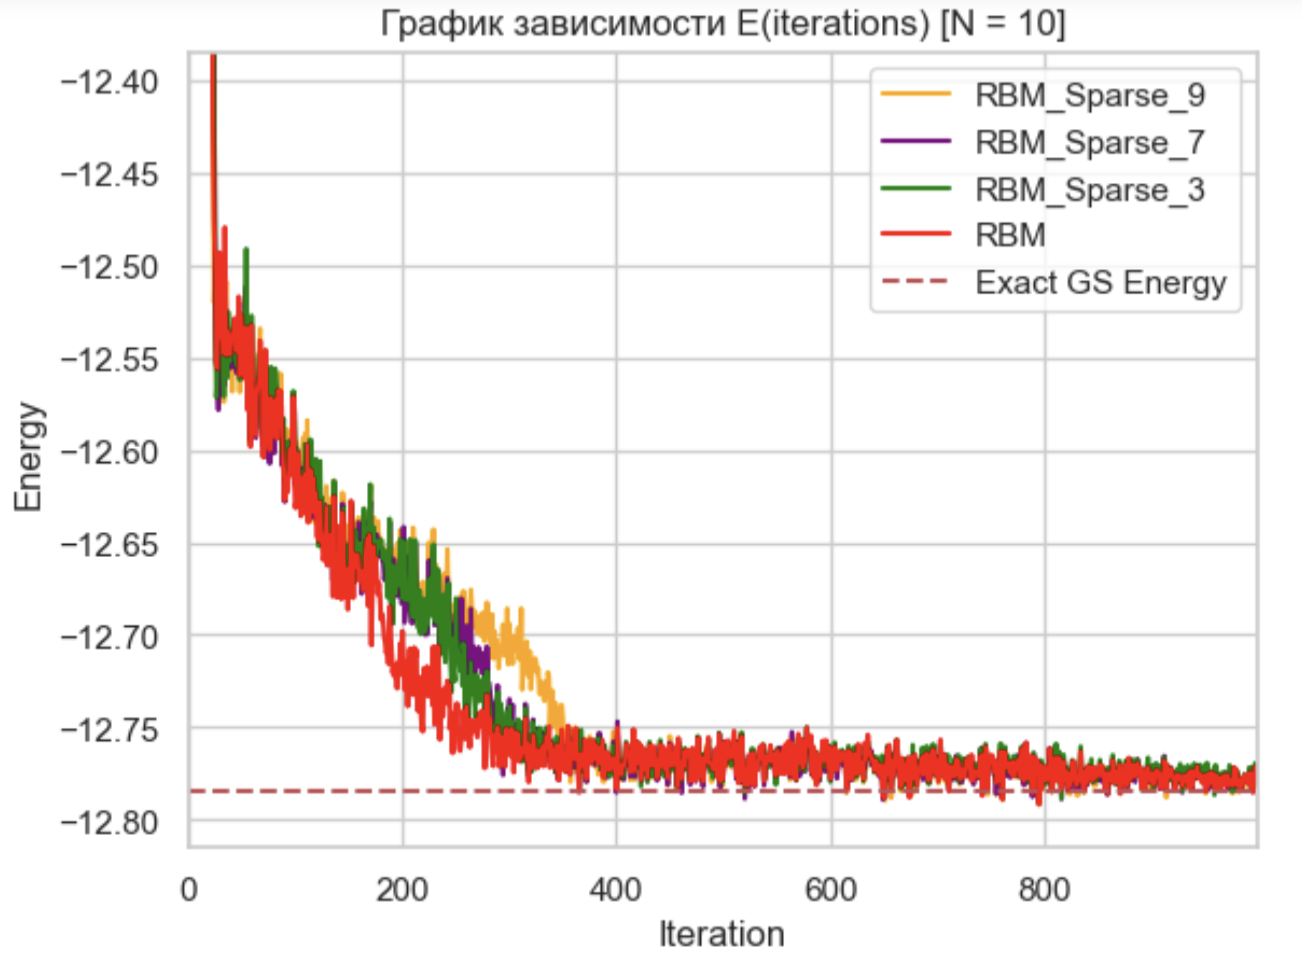
\includegraphics[width=0.50\linewidth]{Course_work/Images/image7.png}
    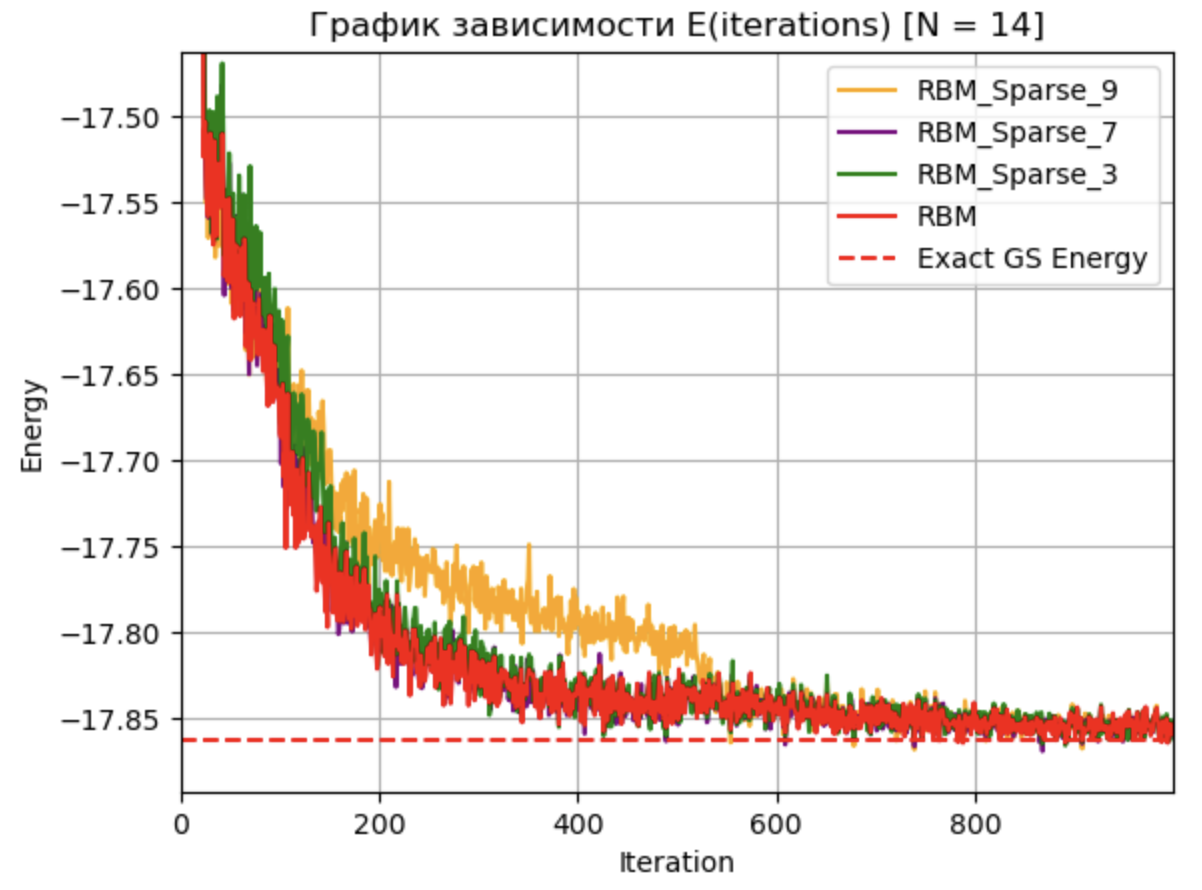
\includegraphics[width=0.50\linewidth]{Course_work/Images/image8.png}
    \caption{}
    \label{fig:e1}
\end{figure}


Как видно из рисунка Рис.\ref{fig:e1} для системы состоящей из 10 спинов быстрее всех сходится обычная RBM, далее RBMSparse3(каждый нейрон входного слоя связан только с 3 нейронами скрытого слоя), далеее RBMSparse7 и RBMSparse9 соответственно. Для системы состоящей из 14 спинов ситуация примерно аналогичная: какого-то преимущества разреженной RBM над обычной мы не наблюдаем.
\vspace{0,25cm}

\subsubsection{Анализ зависимости нормированной энергии основного состояния от напряженности поля}
Эти данные не очень показательны, давайте рассмотрим первый набор наблюдаемых параметров - E/N(энергию основного состояния, нормированную на число cпинов в рассматриваемой системе, в зависимости от величины усиления внешнего поля h.)
Хорошо видно, что экспериментальные значения сходятся с теоретическими значениями, вычисленными путем диагонализации гамилониана и вычислением его первого собственного значения, как для RBM, так и для RBMSparse.(см. Рис.\ref{fig:e2},Рис.\ref{fig:e3})

Из графиков Рис.\ref{fig:e4}, Рис.\ref{fig:e5} легко заметить, что энергия уменьшается с ростом напряженности поля. Это объясняется тем, что часть энергии возникает из-за взаимодействий между спиновыми участками и внешним магнитным полем. В одномерном случае увеличение параметра сети \(\alpha \equiv \frac{M}{N}\)\ , т.е. соотношения числа скрытых и явных узлов \(N\), практически не влияет на величину и точность энергии, но время вычислений растет линейно с ростом \(\alpha\).


\begin{figure}[H]
    \centering
    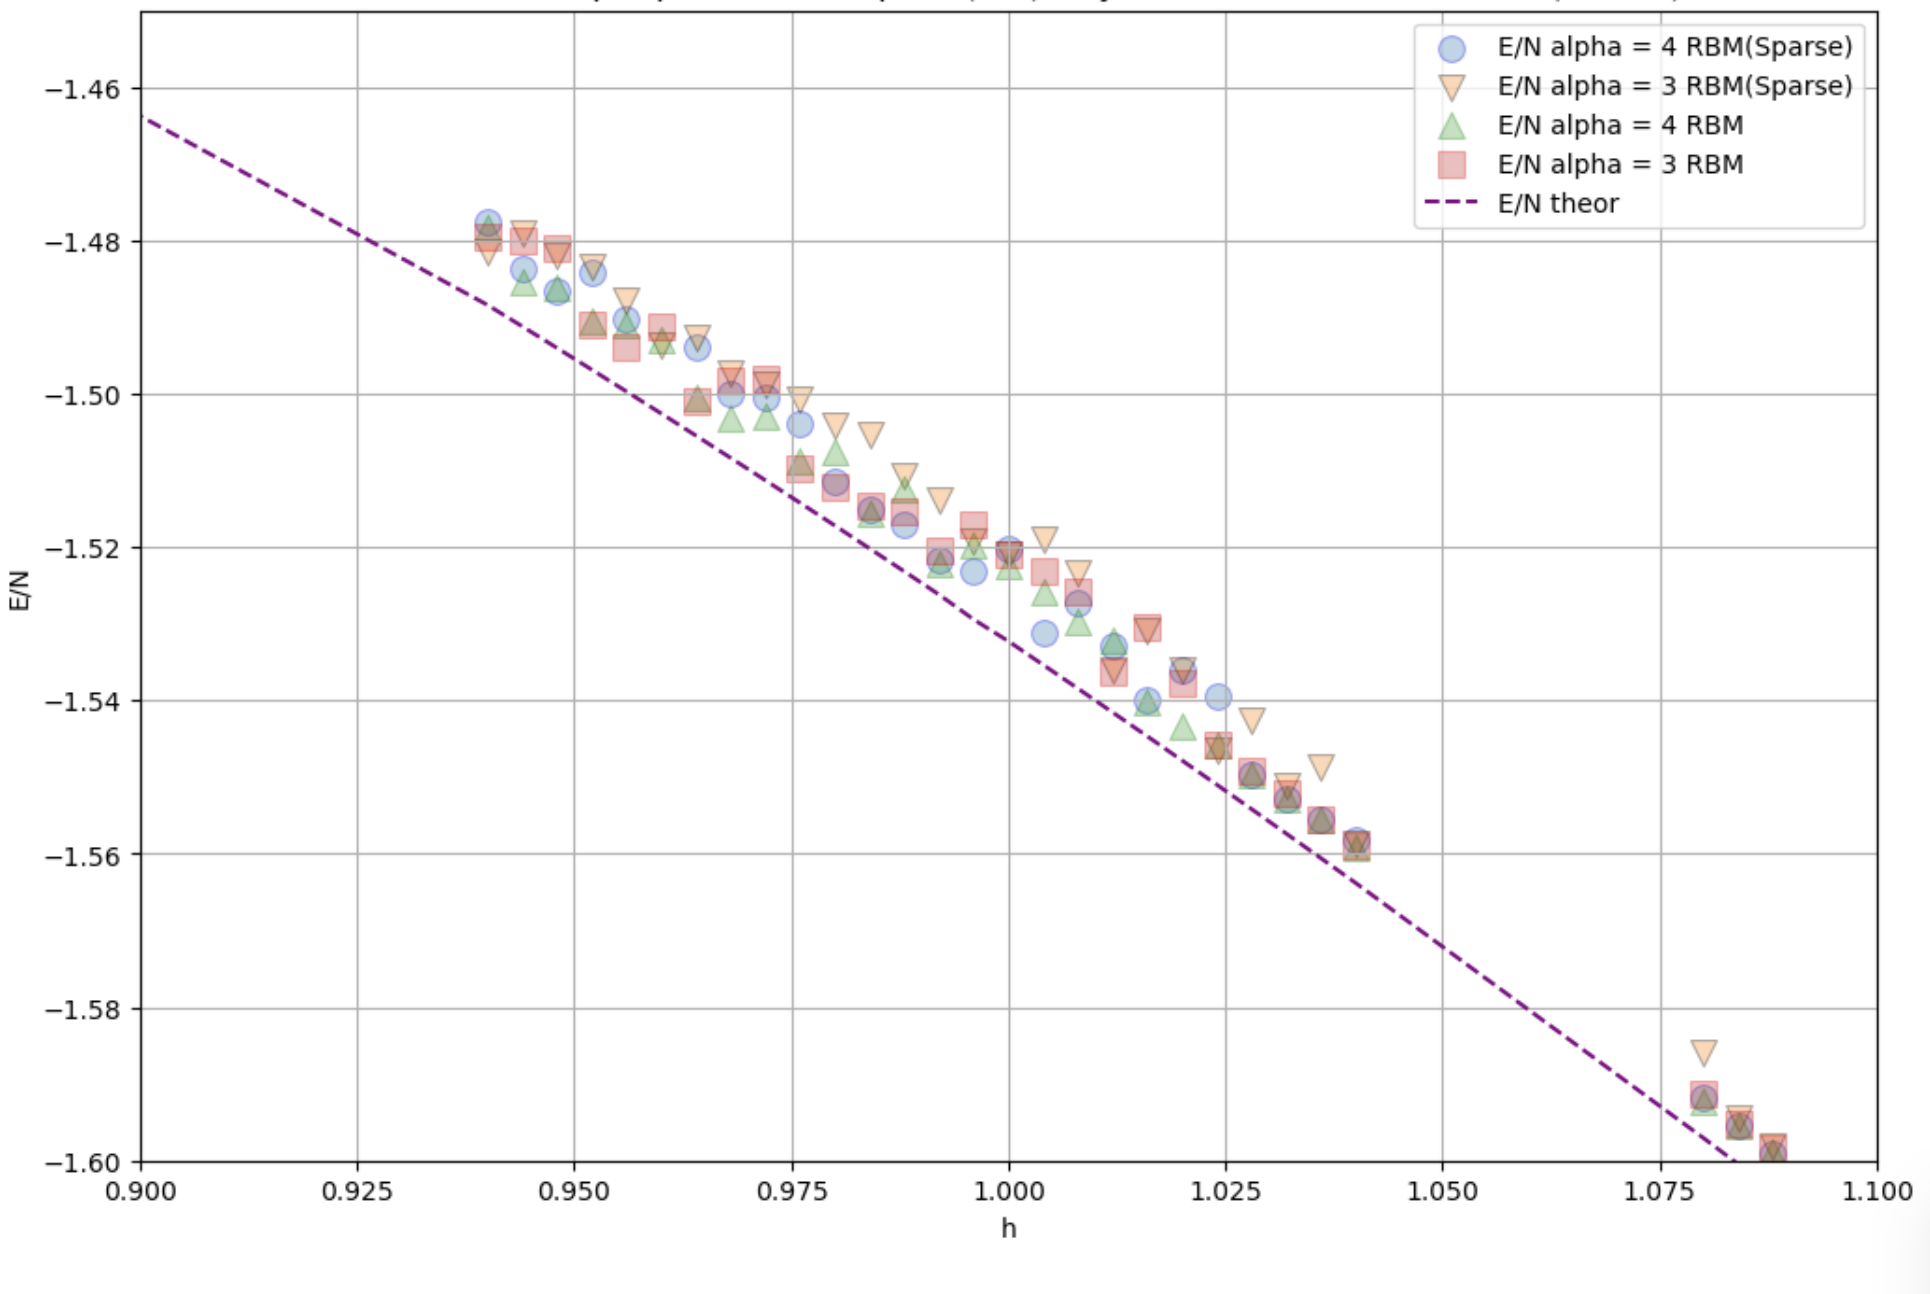
\includegraphics[width=0.8\linewidth]{Course_work/Images/E-N-10-z.png}
    \caption{\textbf{Зависимость E/N (h) в увеличенном масштабе(N=10)}}
    \label{fig:e2}
\end{figure}

\begin{figure}[H]
    \centering
    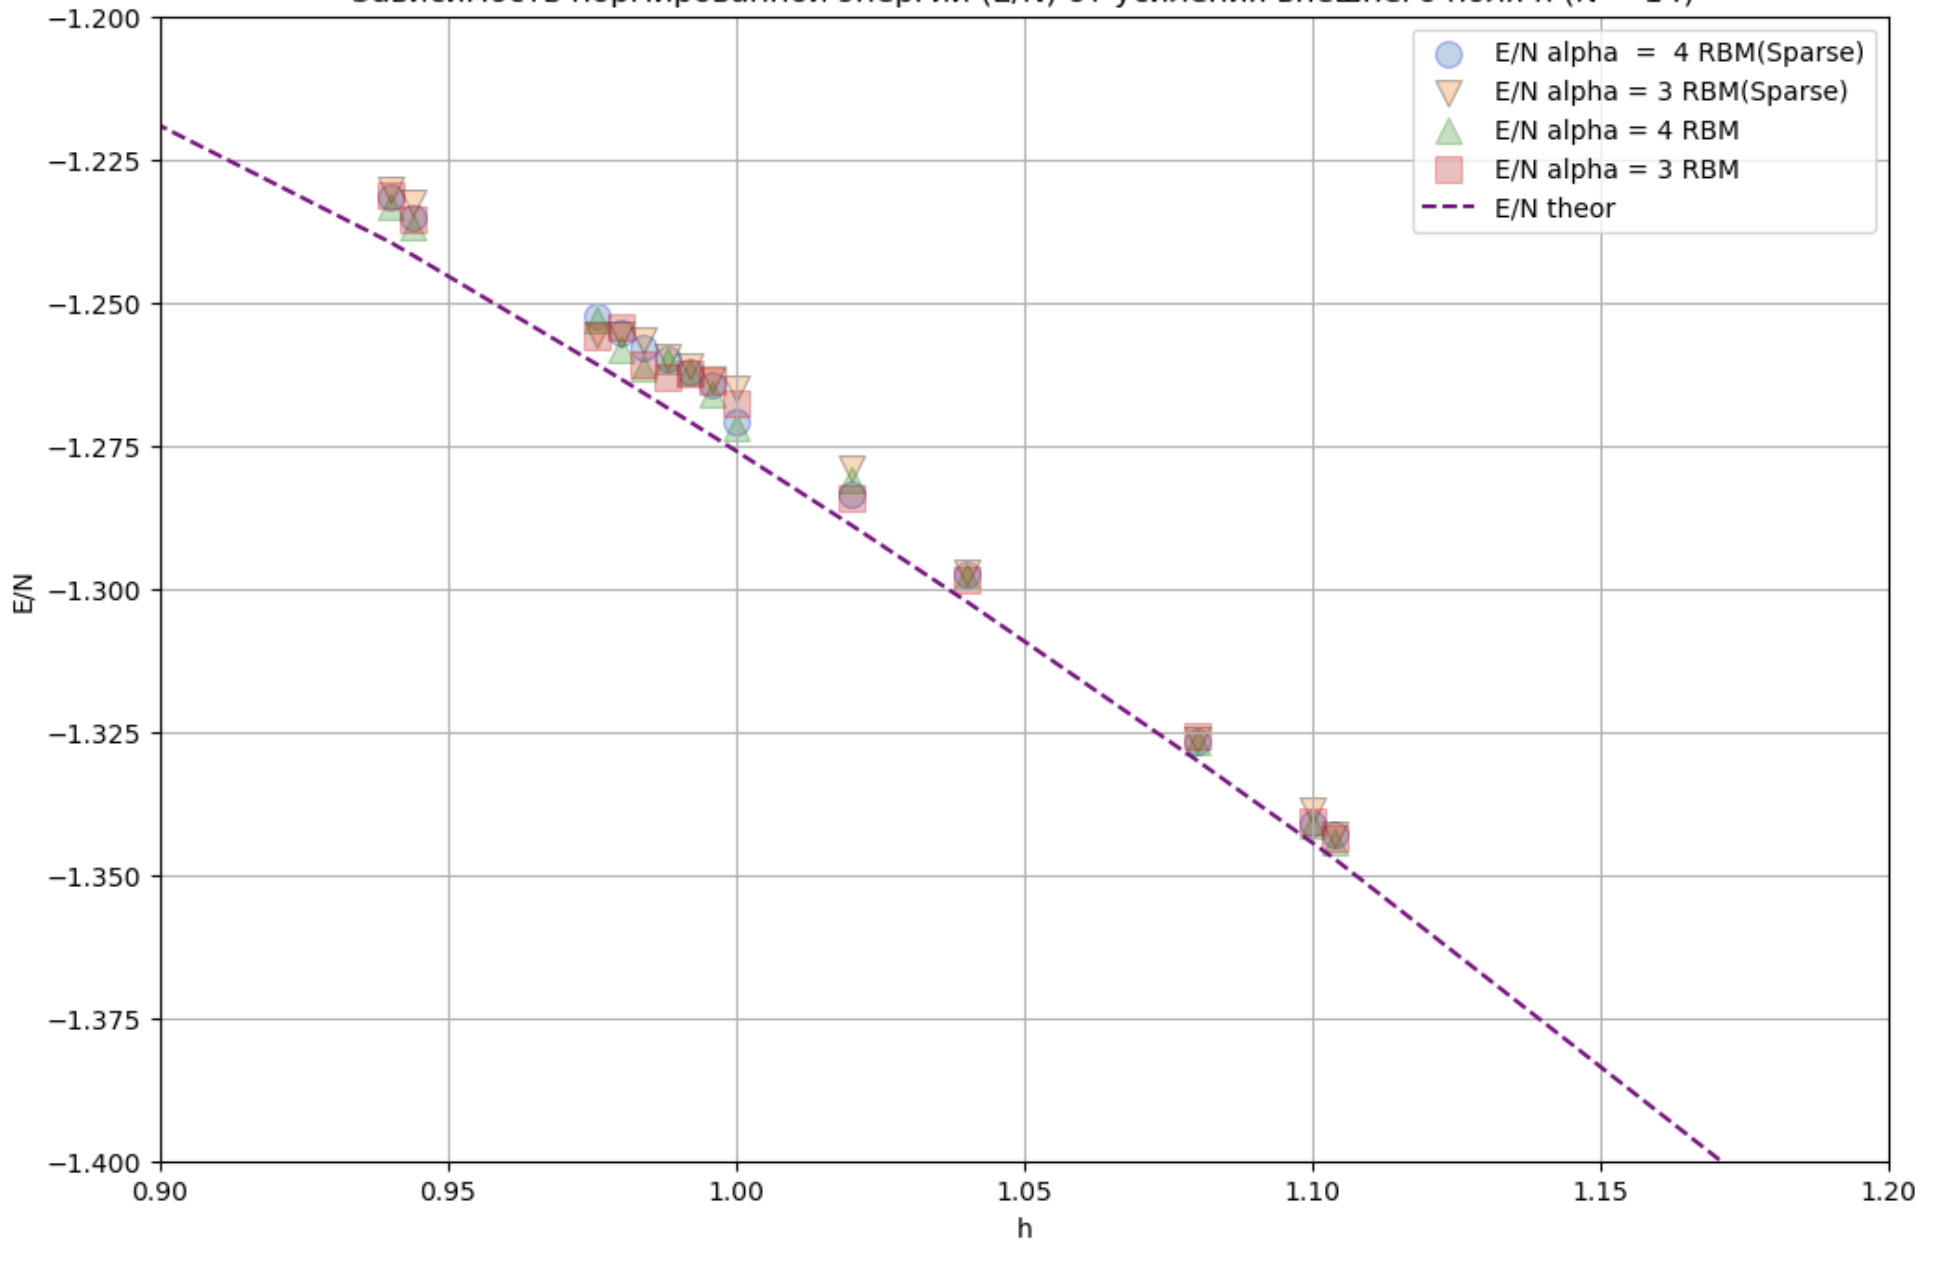
\includegraphics[width=0.8\linewidth]{Course_work/Images/E-N-14-z.png}
    \caption{\textbf{Зависимость E/N (h) в увеличенном масштабе(N=14)}}
    \label{fig:e3}
\end{figure}

%
 %  \begin{figure}[H]
  %      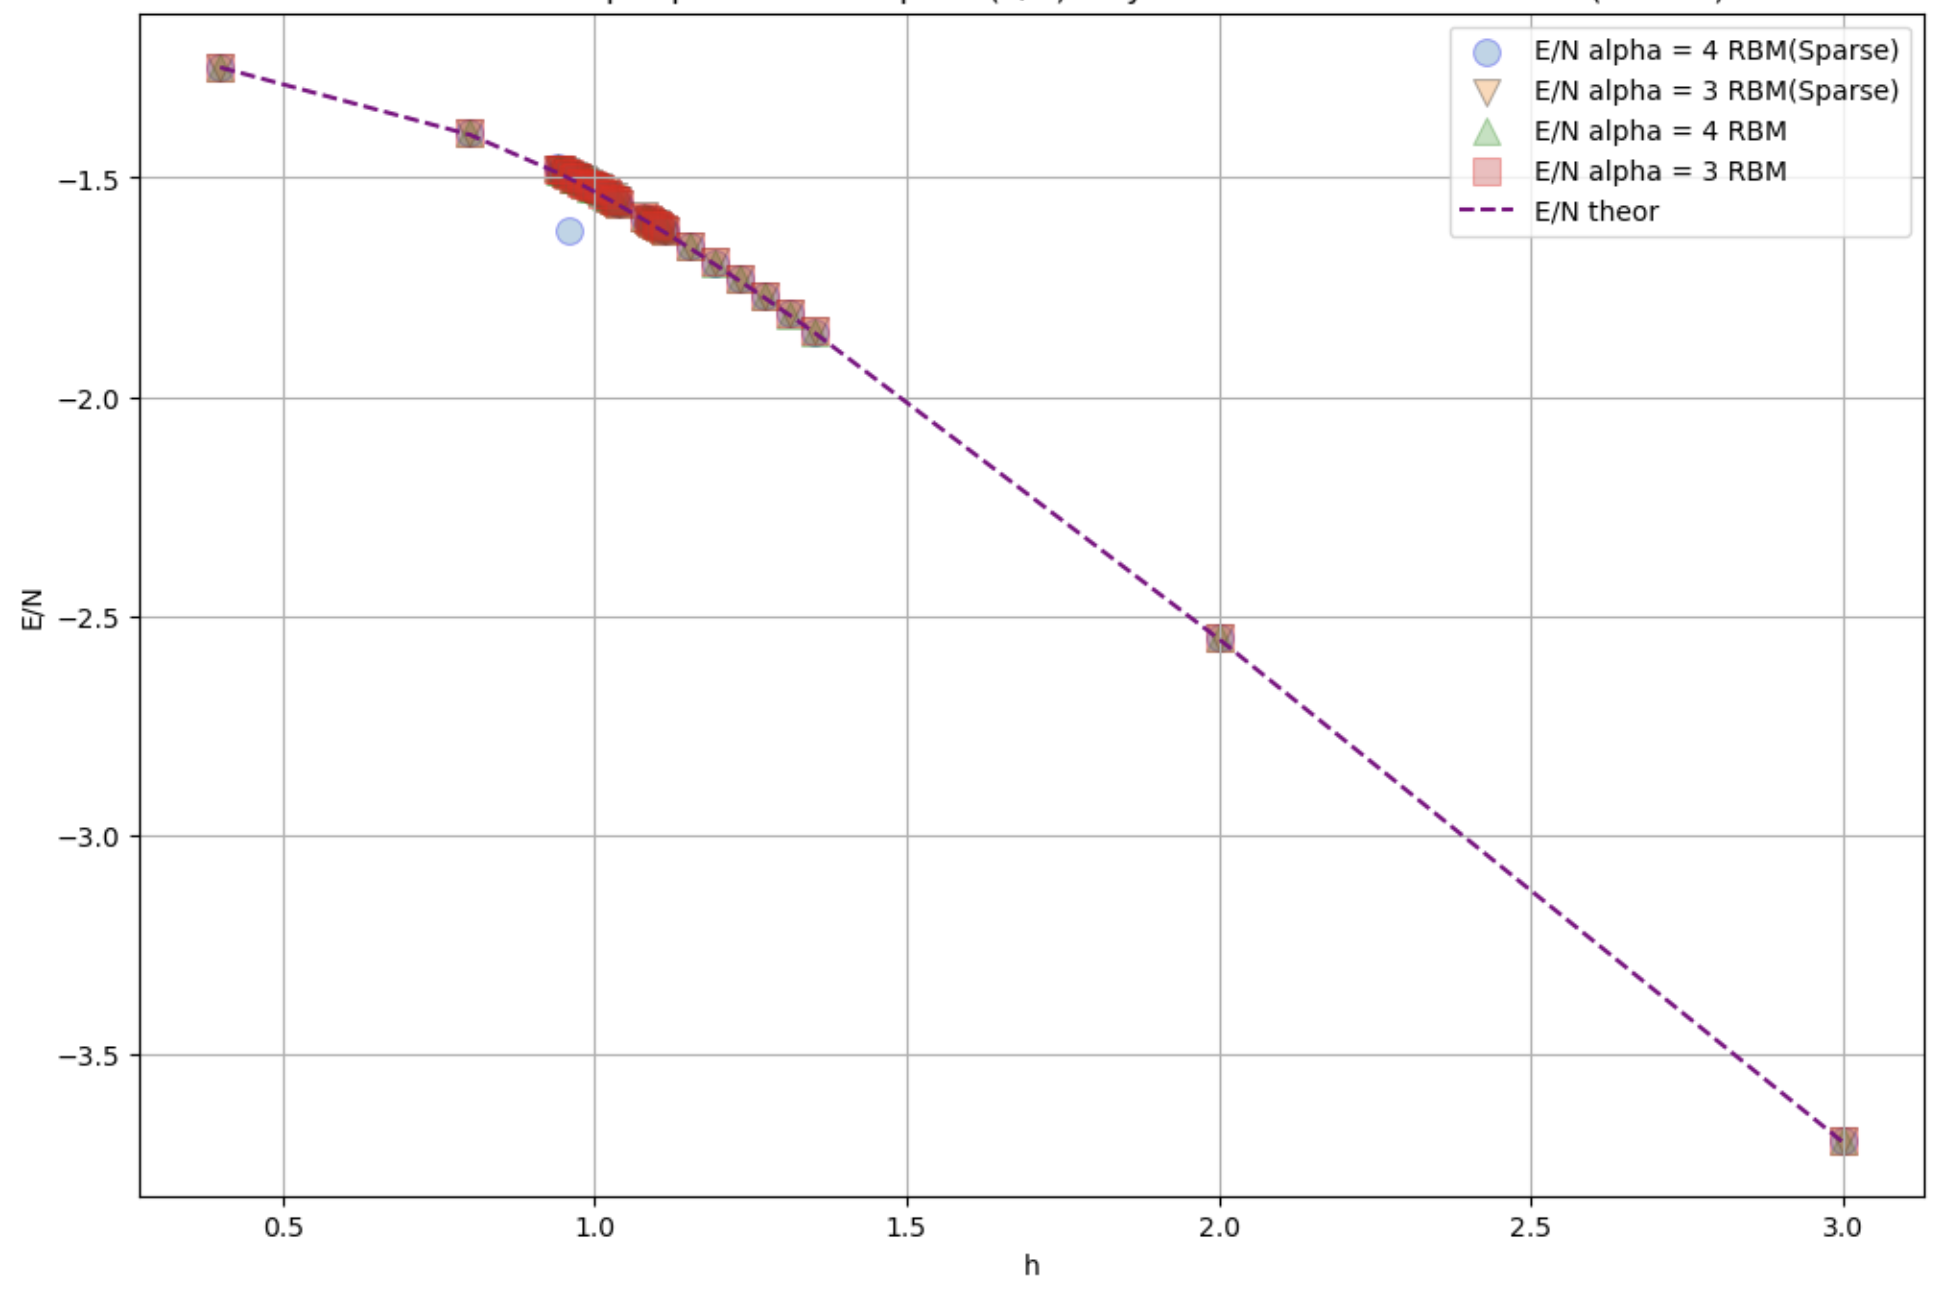
\includegraphics[width=0.50\linewidth]{Course_work/Images/E-N-10.png}
  %      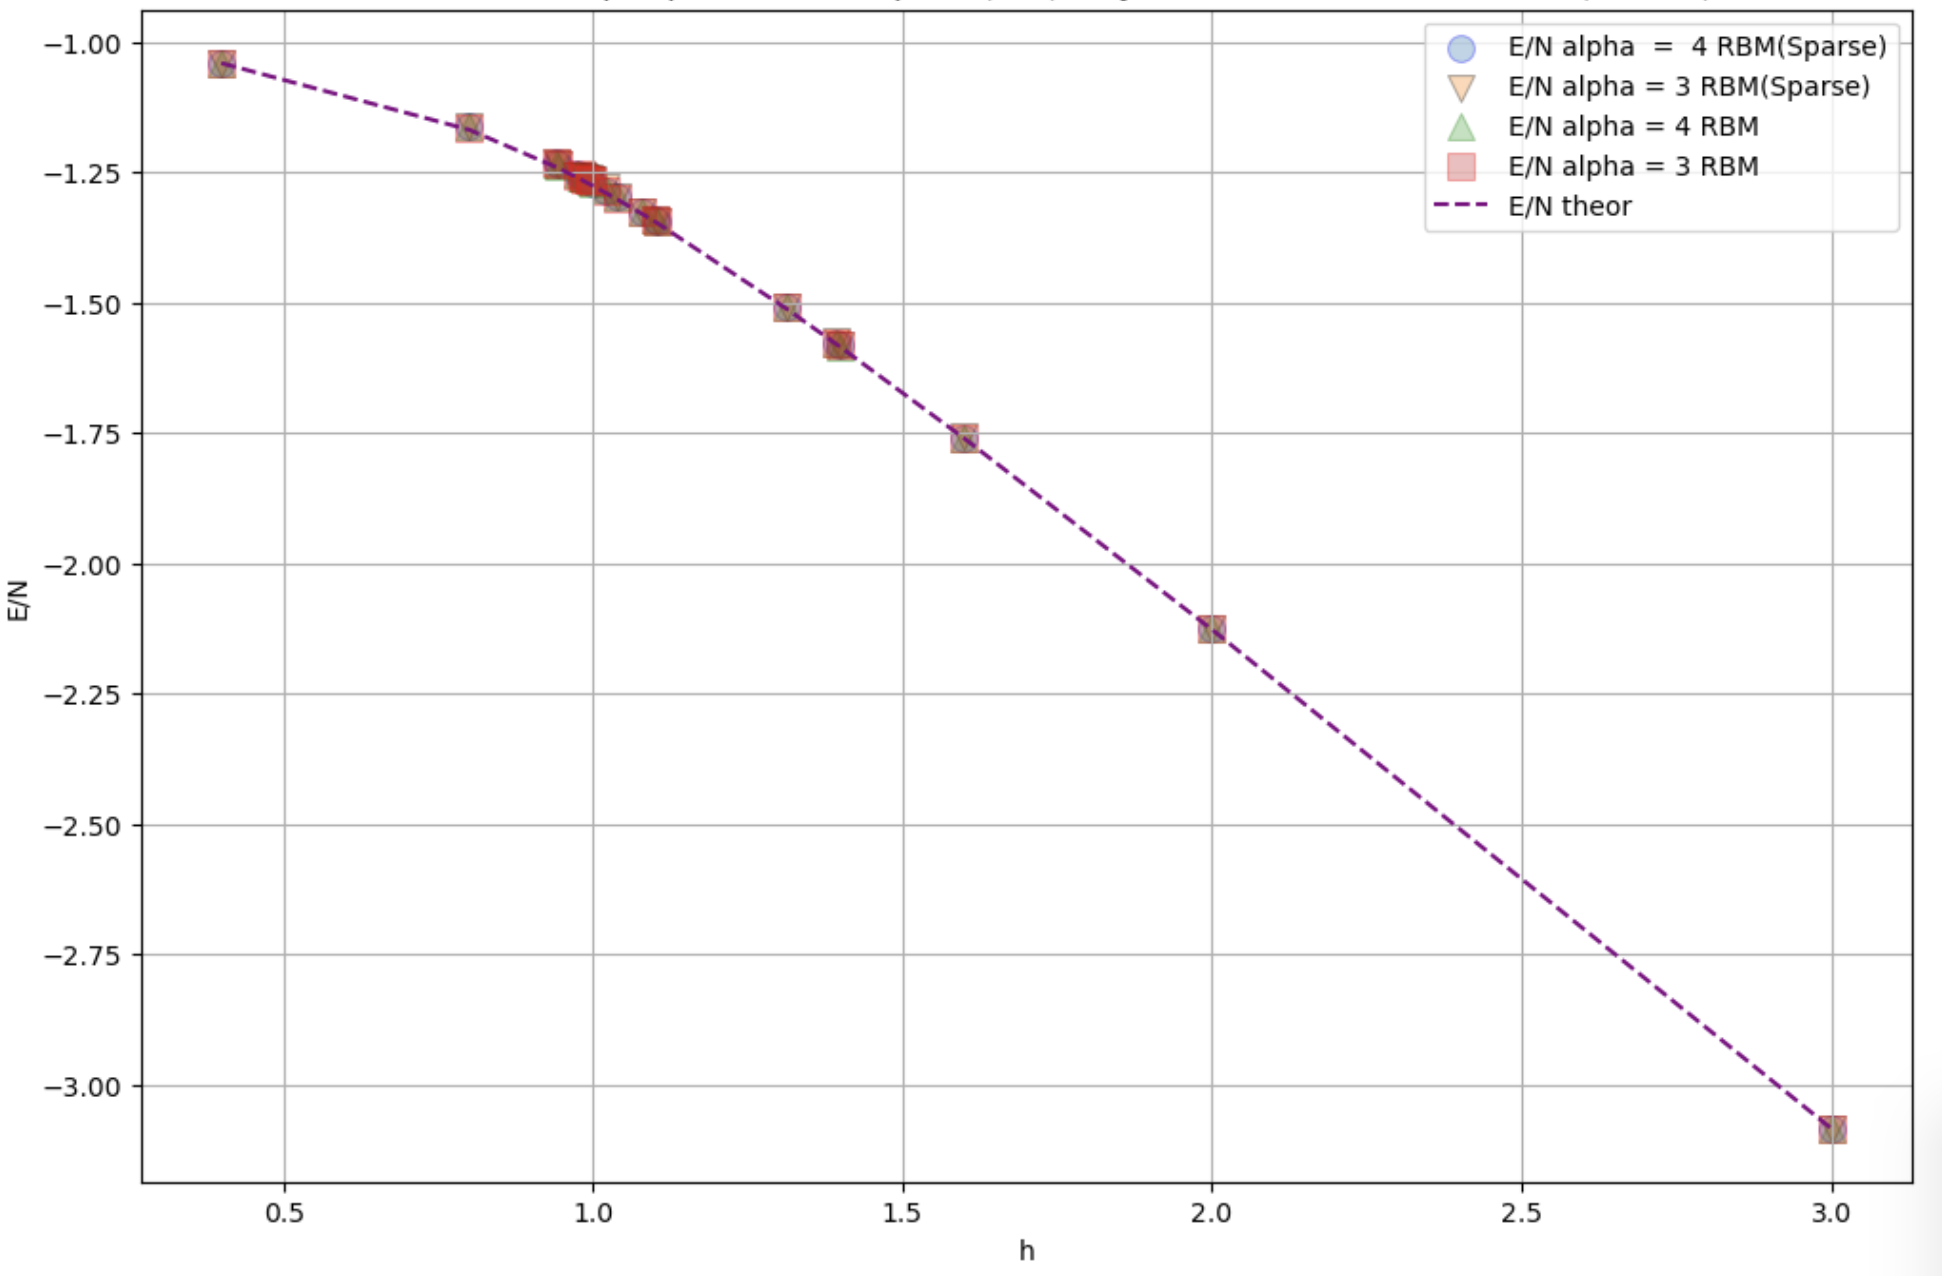
\includegraphics[width=0.50\linewidth]{Course_work/Images/E-N-14.png}
  %      \caption{\textbf{Зависимость нормированной энергии  от напряженности поля(N=10)}}
   %     \label{fig:e1}
%  \end{figure}


\begin{figure}[H]
    \centering
    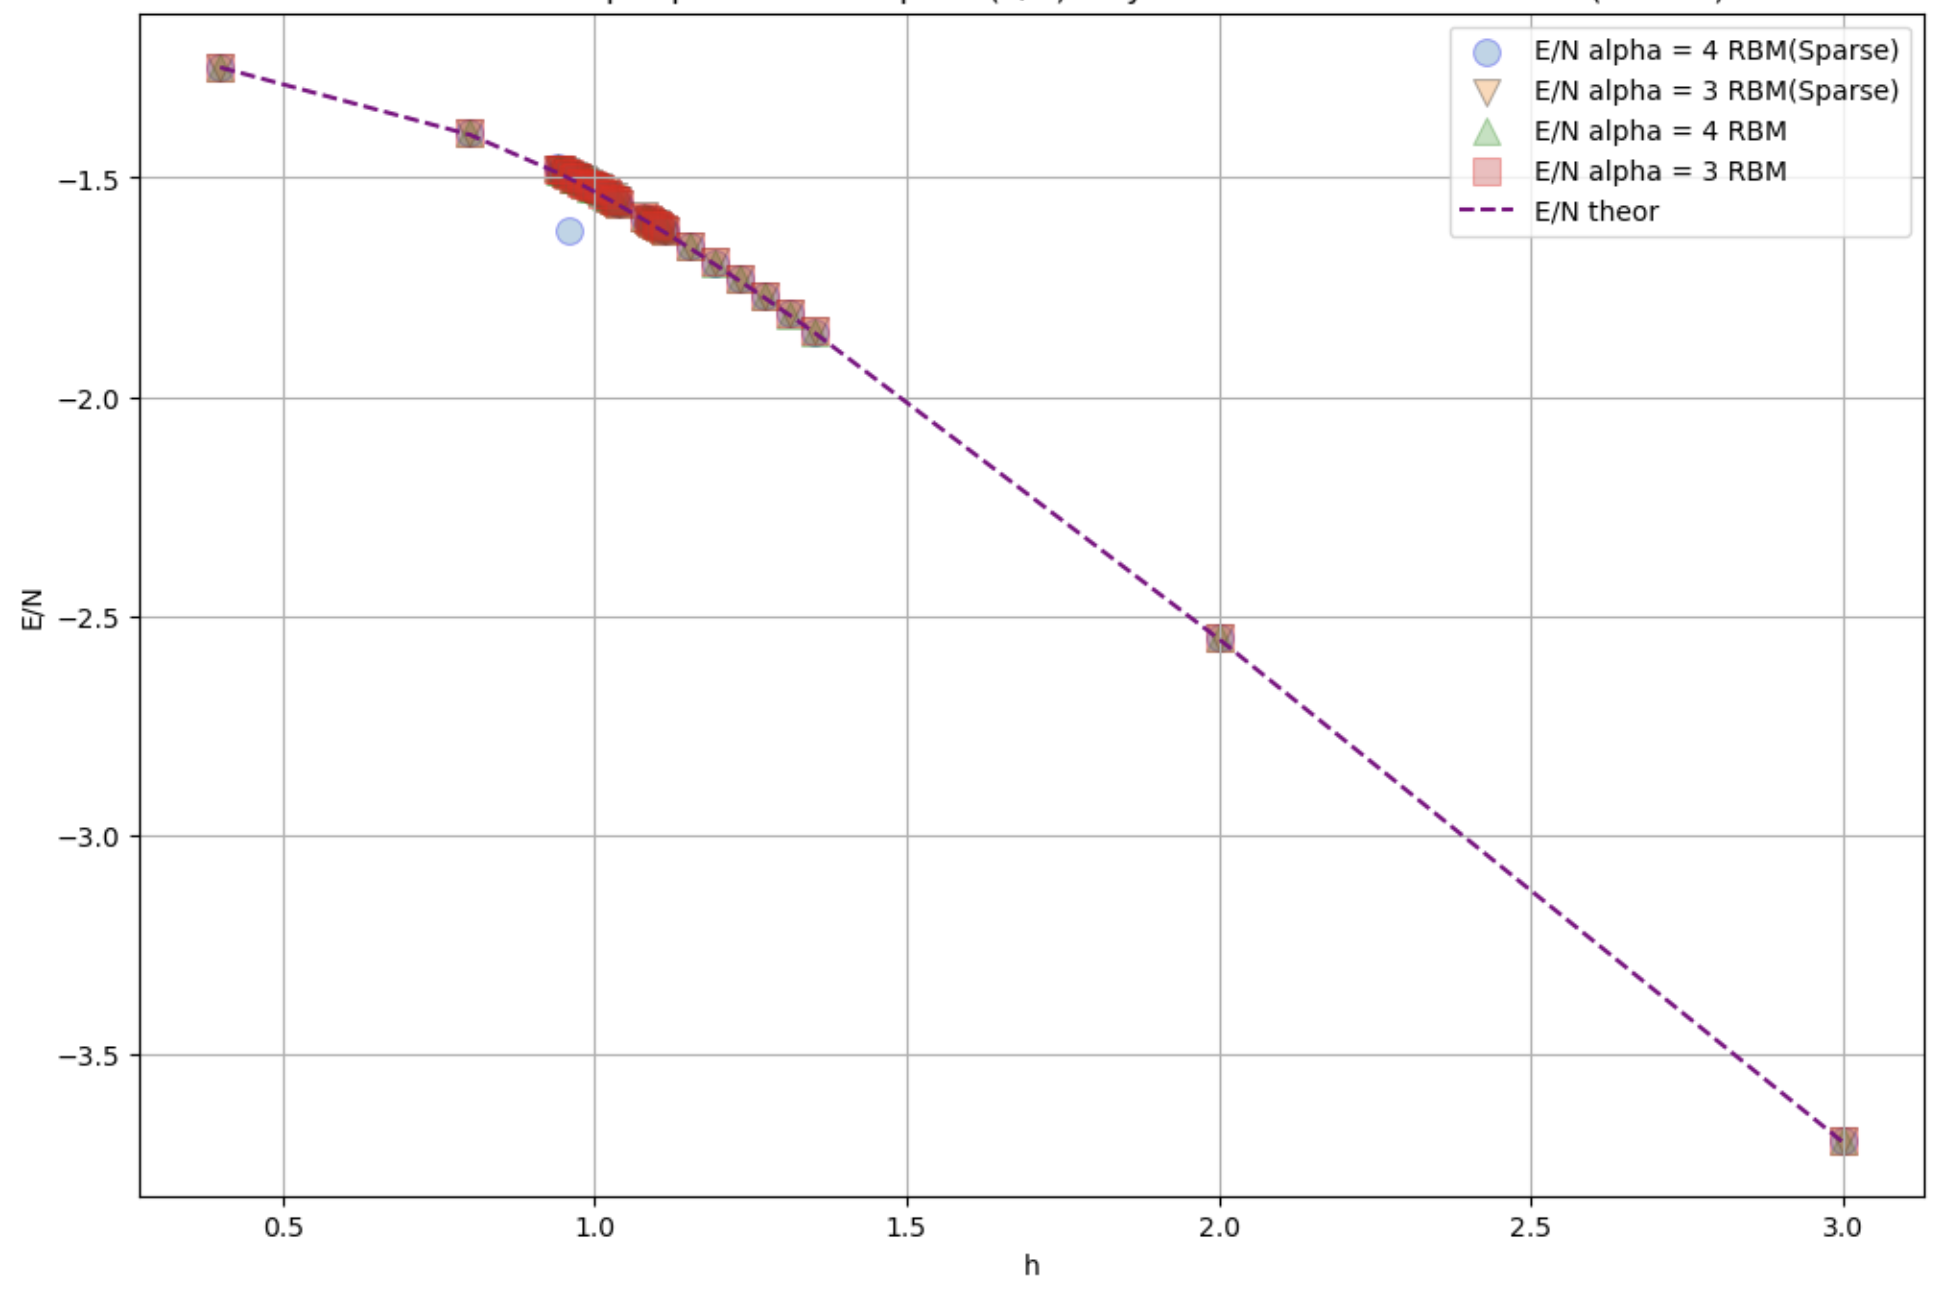
\includegraphics[width=0.8\linewidth]{Course_work/Images/E-N-10.png}
    \caption{\textbf{Зависимость нормированной энергии  от напряженности поля(N=10)}}
    \label{fig:e4}
\end{figure}

\begin{figure}[H]
    \centering
    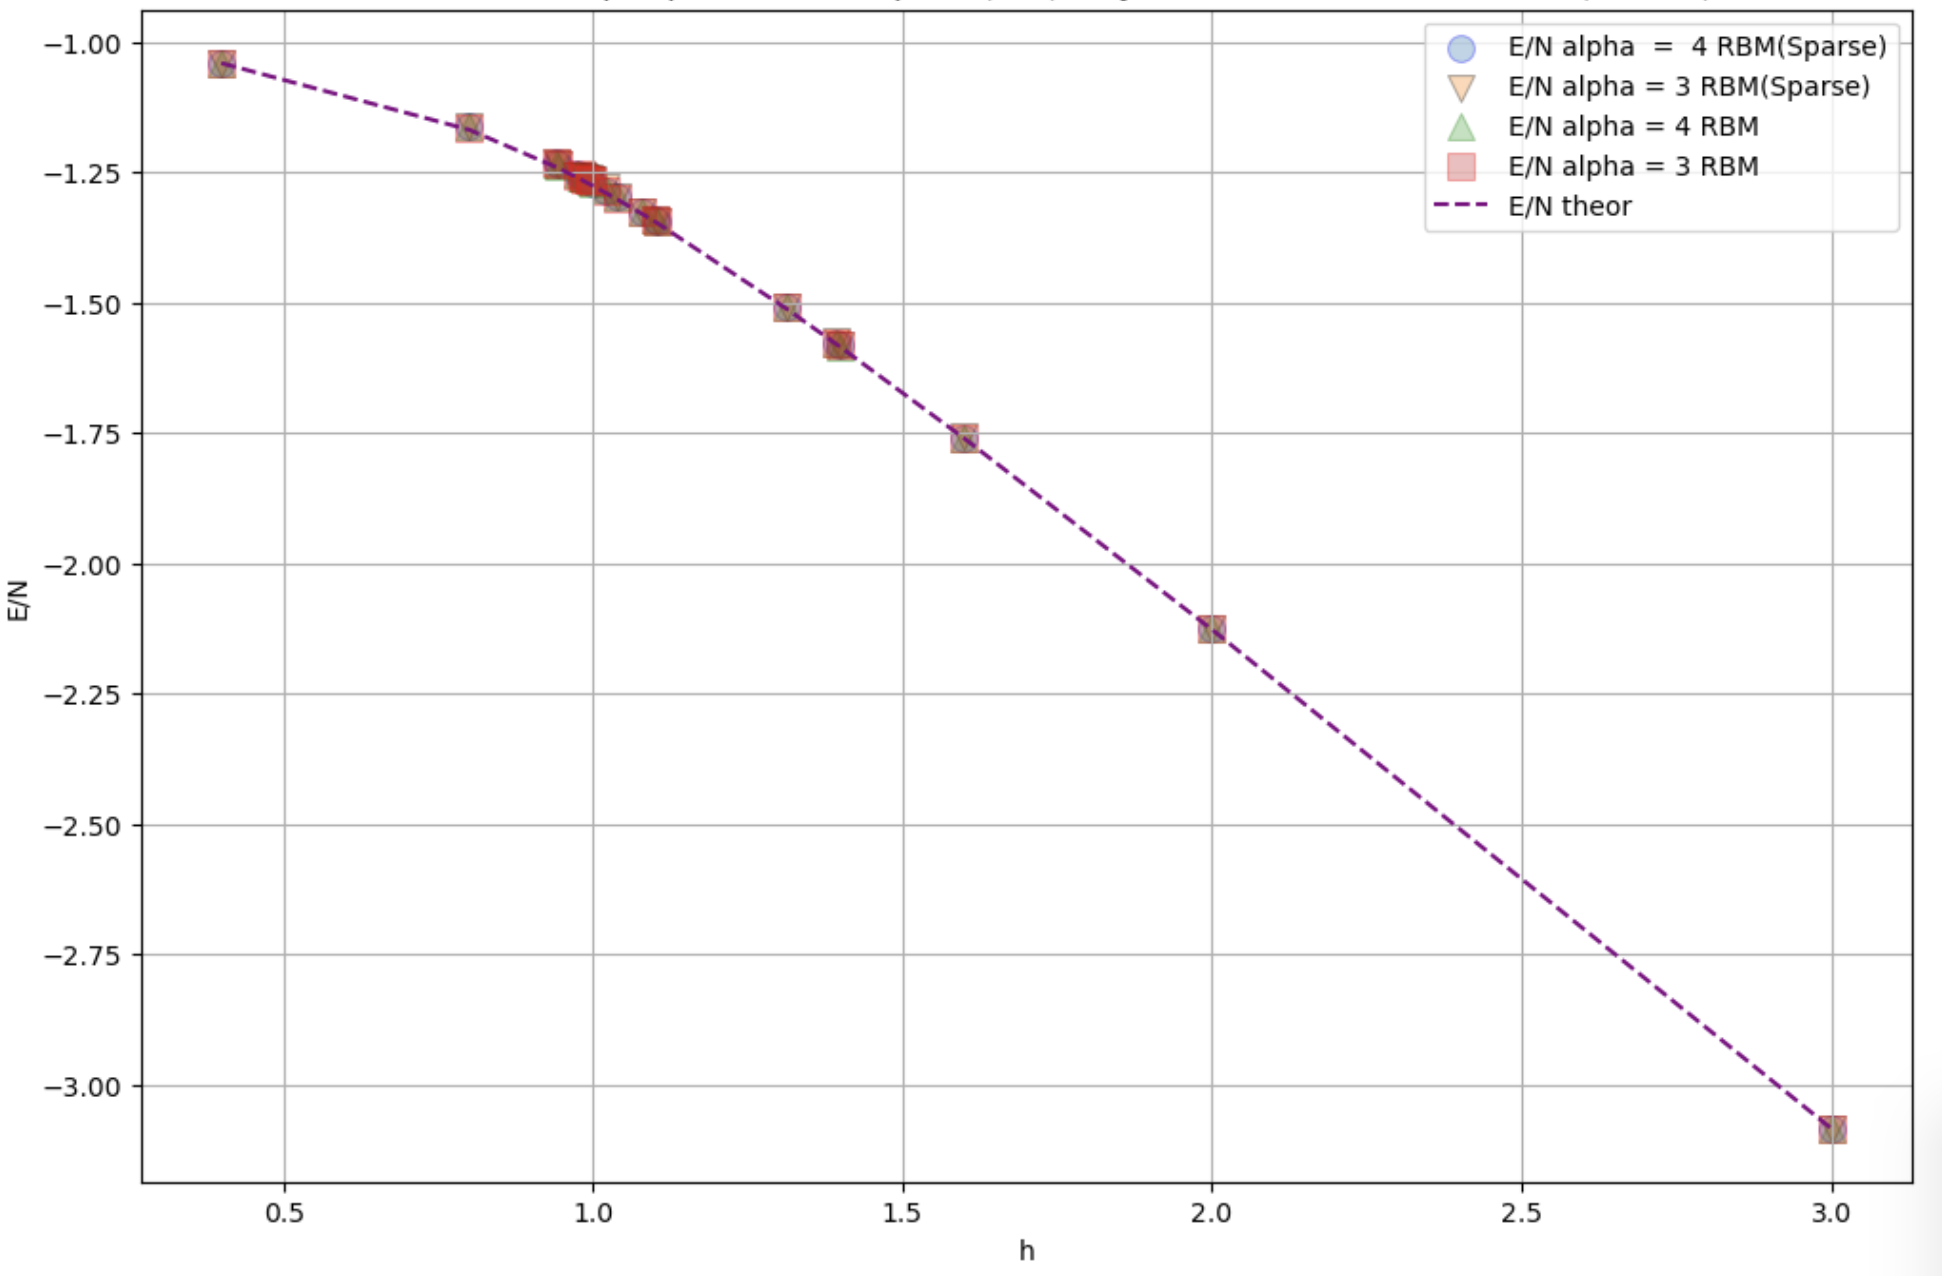
\includegraphics[width=0.8\linewidth]{Course_work/Images/E-N-14.png}
    \caption{\textbf{Зависимость нормированной энергии  от напряженности поля(N=14)}}
    \label{fig:e5}
\end{figure}

\subsubsection{Анализ зависимости спин-z функции коррелятора основного состояния от напряженности поля}

Проведем анализ графика зависимости  функции коррелятора, которая отражает взаимодействие между спинами вдоль выделенной оси z, от напряженности поля для цепочек N = 10 и N = 14.
Сама функция коррелятора считается по формуле $\langle \sigma_i^z \sigma_{i+x}^z \rangle$, усреднение берется по x.

\begin{figure}[H]
    \centering
    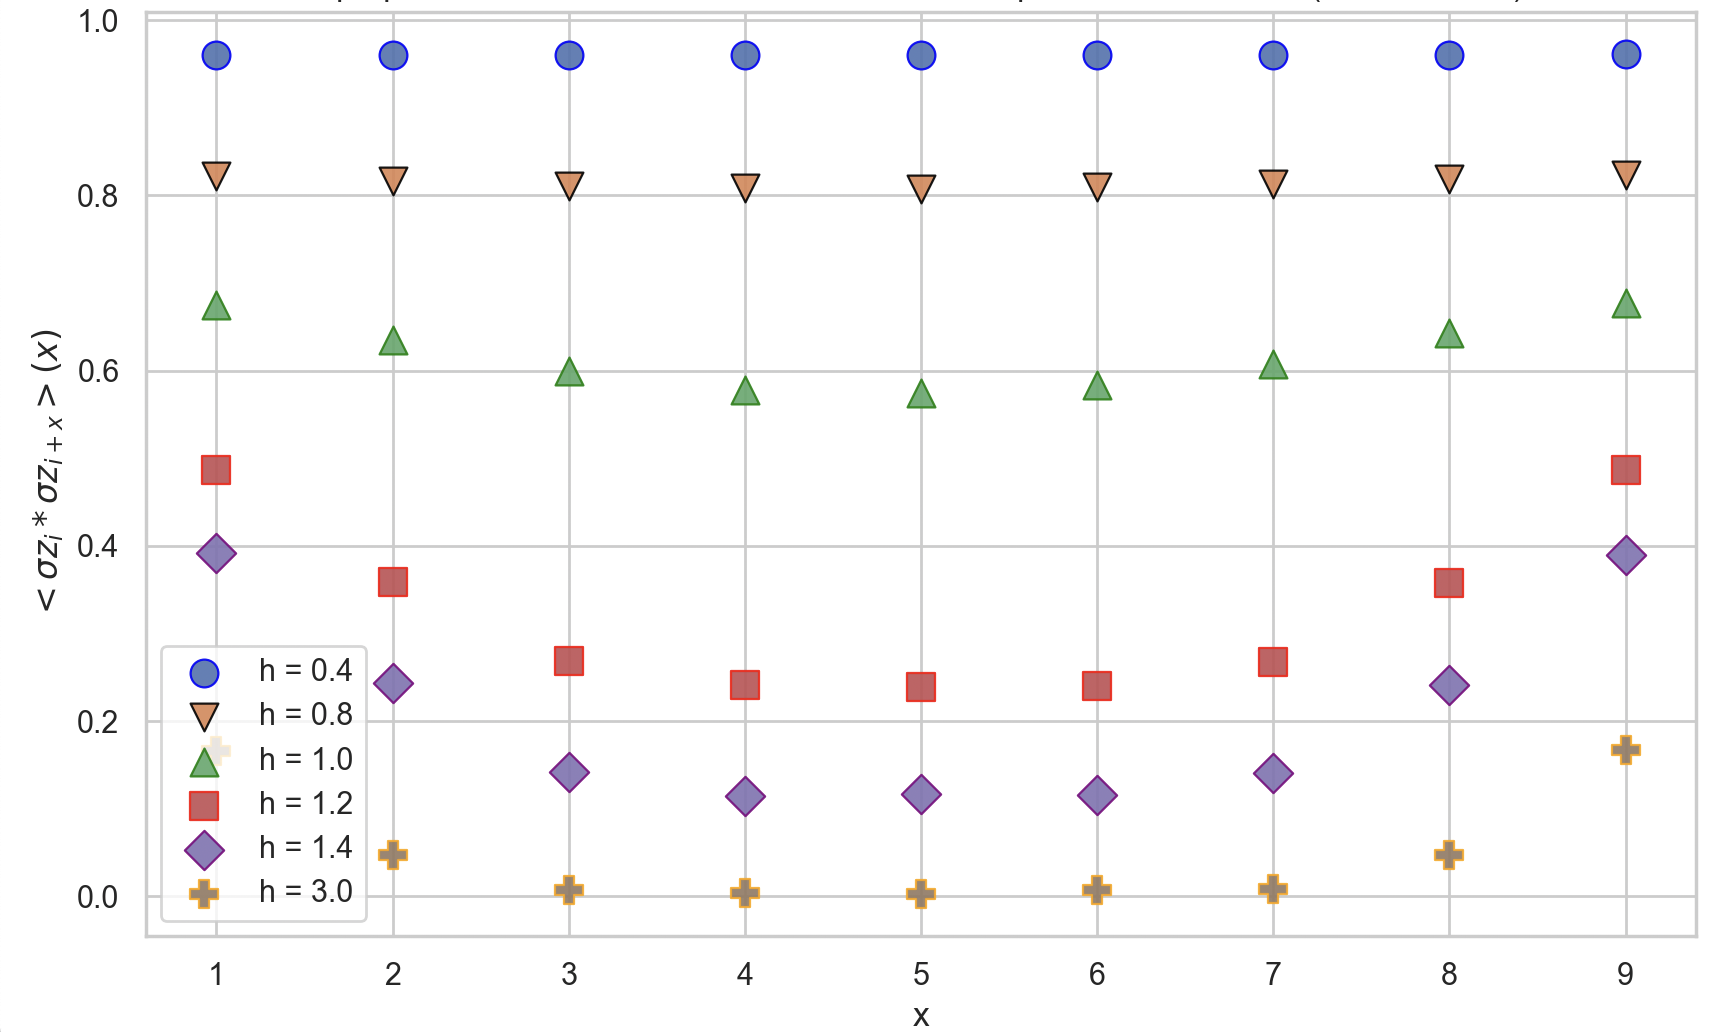
\includegraphics[width=0.8\linewidth]{Course_work/Images/Corr-N-10.png}
    \caption{\textbf{Зависимость спин-z функции коррелятора  от напряженности поля(N=10)}}
    \label{fig:e6}
\end{figure}

\begin{figure}[H]
    \centering
    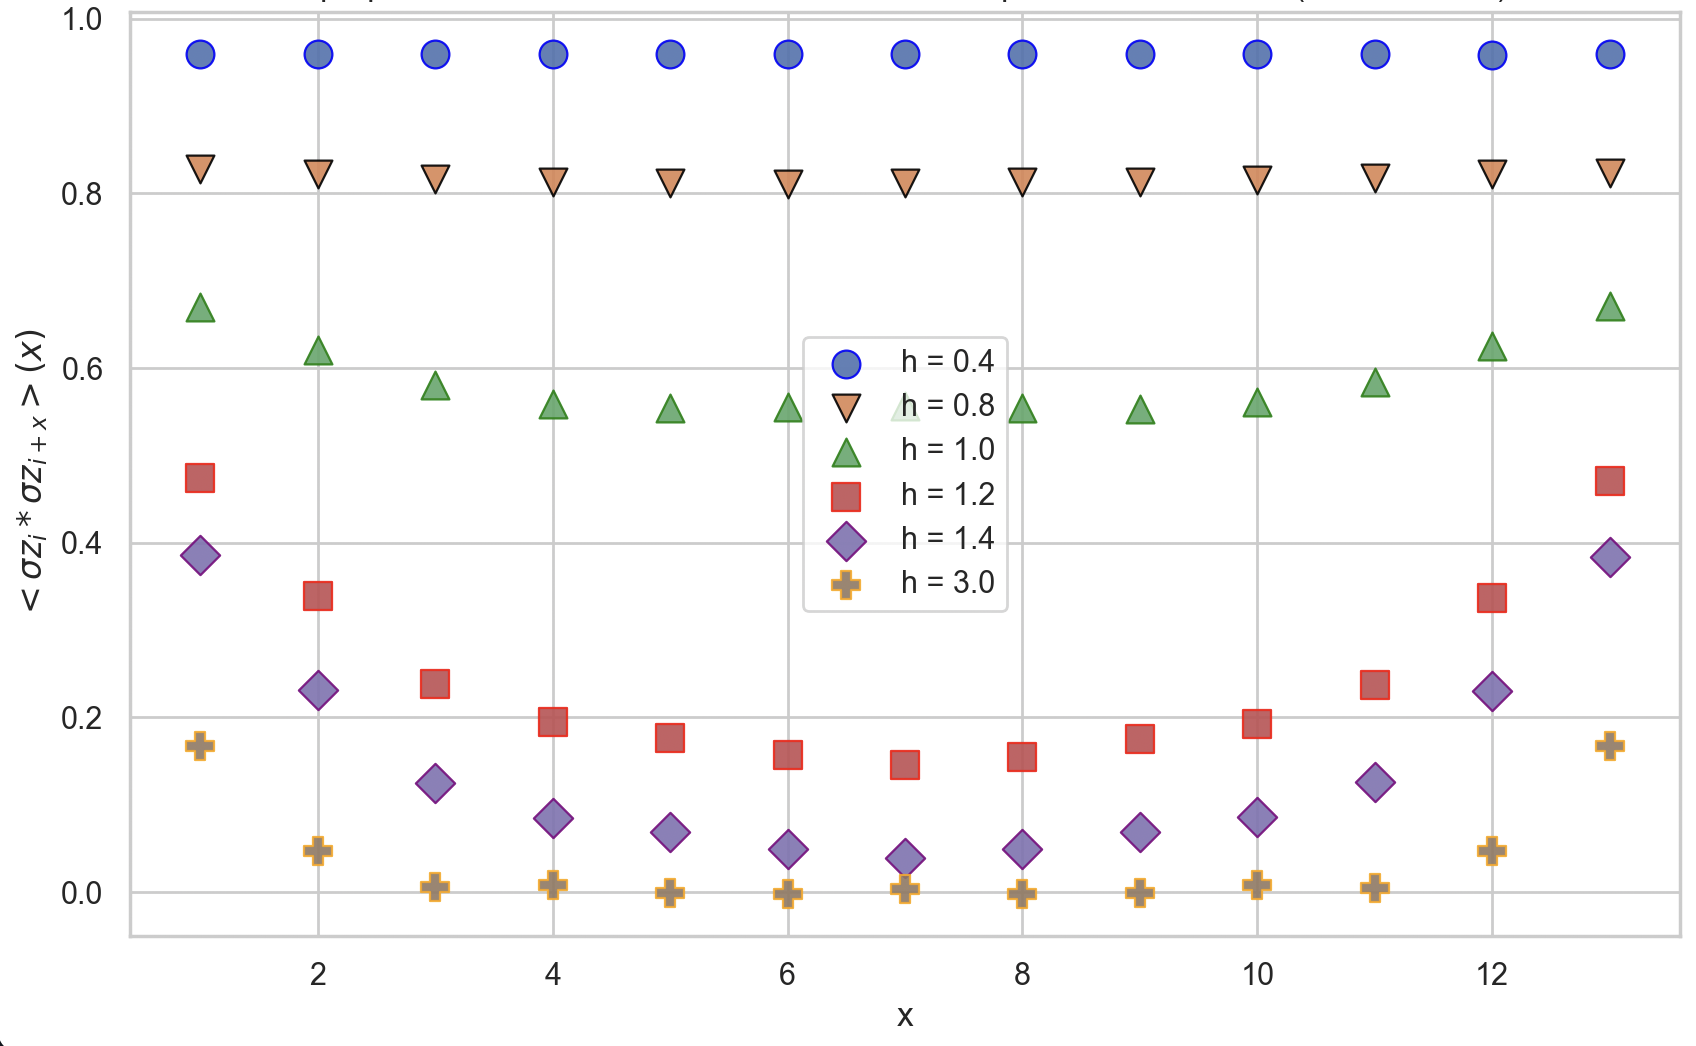
\includegraphics[width=0.8\linewidth]{Course_work/Images/Corr-N-14.png}
    \caption{\textbf{Зависимость спин-z функции коррелятора  от напряженности поля(N=14)}}
    \label{fig:e7}
\end{figure}
Глядя на графики Рис.\ref{fig:e6} и Рис.\ref{fig:e7}) видно, что при малых h проявляется дальнодействующая корреляция.
При увеличии величины напряженности поперечного поля h наступает момент, когда наблюдается скачок корреляционной функции при некотором 
\(h_{\text{кр}} \) = 1.0, в этот момент происходит квантовый фазовый переход 2-го рода во время которого идёт перестройка системы. Этот переход осуществляется в отсутствии тепловых флуктуаций, то есть при изменении внешних нетепловых параметров, в данном случае напряженности поперечного поля. Тут важно сделать оговорку, что на самом деле этот переход происходит при некотором критическом отношении \( \frac{h}{J} \), но в данной работе я положил J = 1. Вообще с точки зрения физики, параметры h и J являются взаимообратными величинами: первое из них стремится нарушить порядок в решетке, а другая наоборот его сохранить.Результаты хорошо согласуются с тем, что получили авторы статьи \cite{shi2021}. 

\subsubsection{Анализ зависимости среднего значения магнитного момента и восприимчивости от  напряженности поля}

Третим набором исследуемых параметров, будет составляющая магнитного момента вдоль напряженности поперечного поля и соответствующая ему магнитная восприимчивость: \begin{equation}
\langle M_x \rangle = \sum_i \langle \psi | \sigma_i^z | \psi \rangle / N, \quad \chi = \lim_{\Delta \to 0} \frac{M_x(h + \Delta) - M_x(h)}{\Delta}
\end{equation}

Из графиков Рис.\ref{fig:e8}, Рис.\ref{fig:e9} видно, что поначалу величина магнитного момента возрастает и при достижении \(h_{\text{кр}} \) наступает озвученный выше  фазовый переход 2-го рода и при дальнейшем увеличении напряженности поперечного поля он достигает некоторого состояния насыщения. Причём отчетливо видно, что для системы с N = 14 спинами RBMSparse оказывает преимущество над обычной RBM в плане точности значений, но при меньшем N = 10, как такового выйгрыша в точности мы не наблюдаем - у RBM она выше. В принципе, на основе этого можно сделать промежуточный вывод о том, что для систем с достаточно большим количеством спинов и параметре кучности \(\alpha \), разреженная RBM(RBMSparse) может конкурировать со стандартной RBM, экономя затраты по используемым вычислительным ресурсам компьютера во время обучении модели, так как количество параметров у неё вместо \(N \times N\) равно \(\sum_i k_i \times N\), где \(k_i\) - количество связей между выделенным \(i\)-м нейроном входного слоя и нейронами скрытого слоя. Это может позволить исследовать параметры систем большей размерности.
\begin{figure}[H]
    \centering
    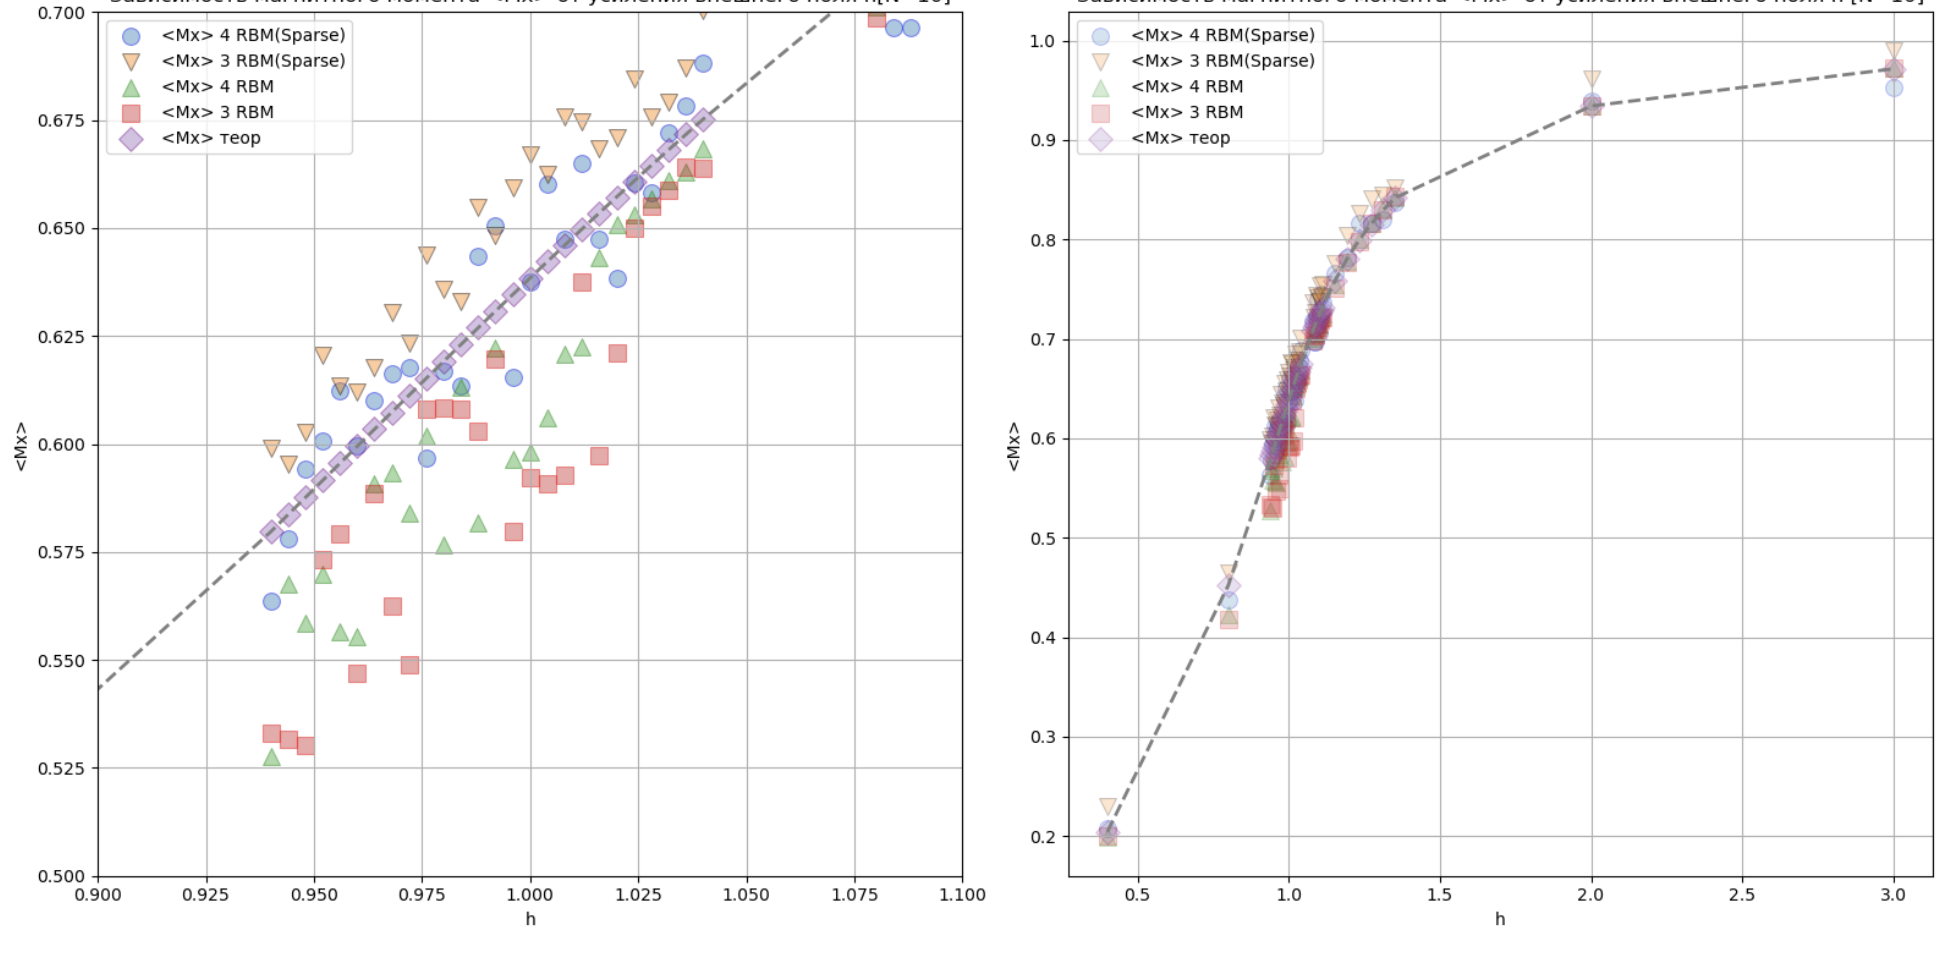
\includegraphics[width=1\linewidth]{Course_work/Images/Mm-N-10.png}
    \caption{\textbf{Зависимость компоненты магнитного поля вдоль напряженности поля от её величины(N=10)}}
    \label{fig:e8}
\end{figure}

\begin{figure}[H]
    \centering
    \includegraphics[width=1\linewidth]{Course_work/Images/MM-N-14.png}
    \caption{\textbf{Зависимость компоненты магнитного поля вдоль напряженности поля от её величины(N=14)}}
    \label{fig:e9}
\end{figure}

Так как магнитная восприимчивость фактически есть производная магнитного момента по h, то \({\Delta} \) нужно выбрать достаточное для того, чтобы правильно получить искомые значения, потому что экспериментальная зависимость не монотонна на каждом рассматриваемом интервале на котором функция непрерывна из-за наличия ошибки модели. По этой причине  при построении зависимости значение \({\Delta} \)  варьировалось от 0,04 до 0,1 и какие-то выводы о точности рассматриваемых моделей сделать сложно. Построенные зависимости показаны на Рис.\ref{fig:e10}, Рис.\ref{fig:e11} .

\begin{figure}[H]
    \centering
    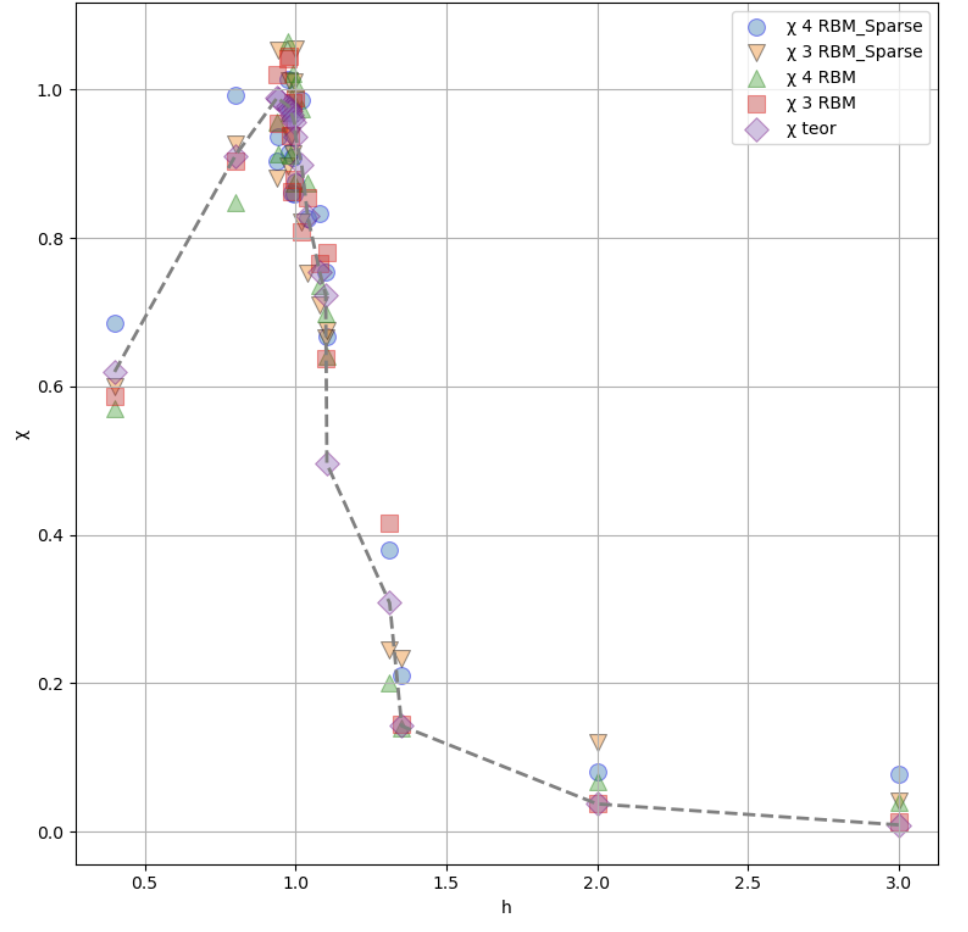
\includegraphics[width=1\linewidth]{Course_work/Images/MV-N-10.png}
    \caption{\textbf{Зависимость магнитной восприимчивости x- компоненты магнитного момента  от напряженности поля(N=10)}}
    \label{fig:e10}
\end{figure}



\begin{figure}[H]
    \centering
    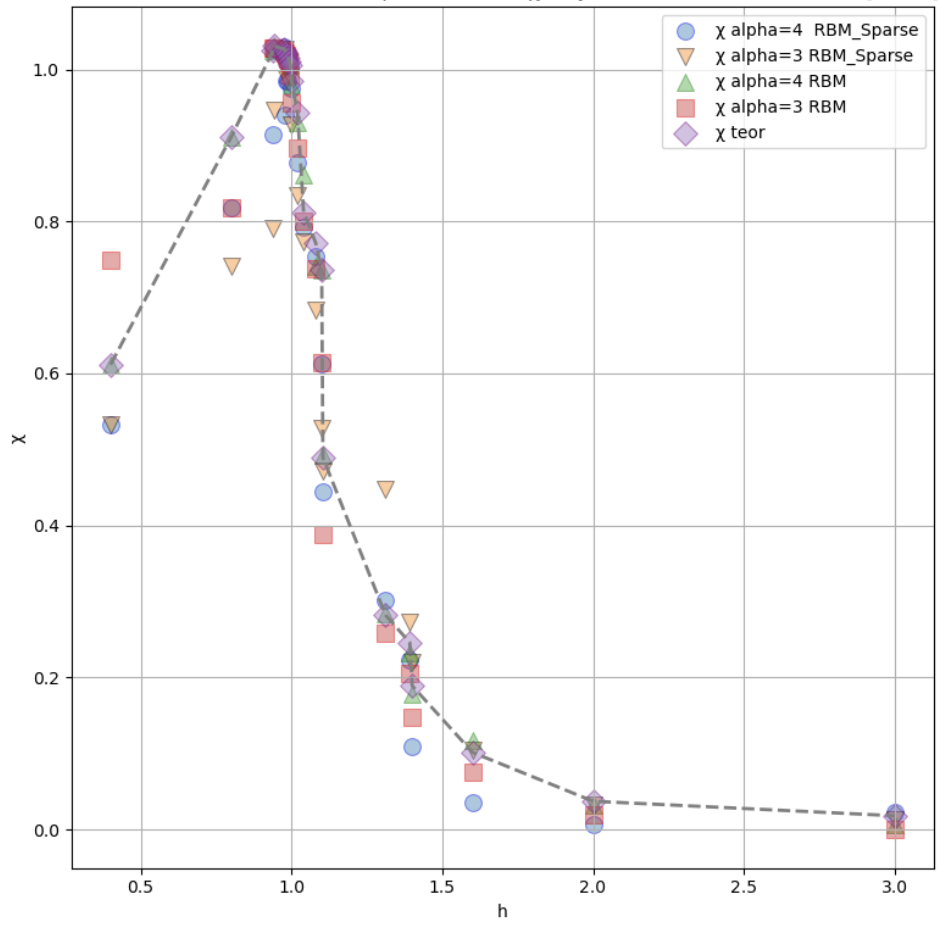
\includegraphics[width=1\linewidth]{Course_work/Images/MV-N-14.png}
    \caption{\textbf{Зависимость магнитной восприимчивости x-компоненты магнитного момента  от напряженности поля(N=14)}}
    \label{fig:e11}
\end{figure}

Здесь мы также видим, что при достижении критического значения h у нас идёт резкое уменьшение магнитной восприимчивости вследствие фазового перехода 2-го рода в ходе которого происходит намагничивание в направлении внешнего поля и как следствие уменьшение магнитной восприимчивости. Это согласуется с  аналитическими данными полученными в \cite{gomes2024} (мы наблюдаем  фазовый переход 2-го рода: ферромагнетик \(\rightarrow\)  парамагнетик).

\section{Подведение итогов}

В данной работе с помощью стандратной ограниченной машины больцмана и разреженной я исследовал параметры системы модели Изинга поперечного поля и провёл соответствующую обработку результатов измерений. Полученные результаты многообещающие - точность разреженной RBM для больших N не уступает точности обычной RBM, а где-то даже её превосходит. Это предоставляет возможность  исследовать параметры системы большей размерности, при этом экономив вычислительные ресурсы компьютера в силу меньшего количества весов, однако из-за ограниченности программного пакета Netket, с которым я работал, приходилось отдельно в цикле занулять веса на каждой итерации обучения модели, ибо установить нужные нам параметры модели во время её инициализации, которые использовались бы при дальнейшем обучении, на данный момент не представляется возможным из коробки пакета. Этот цикл дополнительно увеличивает время работы алгоритма по времени на \(N^2 \times \text{iters} \), где N - размерность системы, а iters - число итераций, поэтому для больших систем процесс обучения может затянуться, но в целом сама концепция прекрасно будет работать при наличии нужного интерфейса.


\newpage
% Список литературы
% Список литературы
\bibliographystyle{plain}
\begin{thebibliography}{9}
    \bibitem{kolmogorov1957} A. N. Kolmogorov, ``On the representation of continuous functions of several variables by superpositions of continuous functions of one variable and addition,'' Doklady Akademii Nauk SSSR, vol. 114, no. 5, pp. 953–956, 1957.
    \bibitem{arnold1963} V. I. Arnold, ``On functions of three variables,'' Doklady Akademii Nauk SSSR, vol. 123, no. 5, pp. 612–614, 1958.
    \bibitem{kolmogorov1936} A. N. Kolmogorov, ``On the representation of continuous functions of many variables by superpositions of continuous functions of one variable and addition,'' Doklady Akademii Nauk SSSR, vol. 108, no. 2, pp. 179–182, 1956.
    \bibitem{shi2021}
    Han-qing Shi, Xiao-yue Sun, and Ding-fang Zeng,
    ``Neural-network Quantum State of Transverse-field Ising Model,''
    Theoretical Physics Division, College of Applied Sciences, Beijing University of Technology.
    \bibitem{melko2020}
    Melko, R. G., Carleo, G., Carrasquilla, J., & Cirac, J. I. (год). Restricted Boltzmann machines in quantum physics. 
    \bibitem{gomes2024}
        Gomes, J., & Eastman, P. (год). Classical Quantum Optimization with Neural Network Quantum States. \textit{Название журнала или конференции}, \textit{том}(выпуск), страницы. 
        
    \bibitem{paramagnetismwiki}
    Paramagnetism. Wikipedia. URL: \url{https://en.wikipedia.org/wiki/Paramagnetism}
    \bibitem{qubitwiki}
    Qubit. Wikipedia. URL: \url{https://en.wikipedia.org/wiki/Qubit}
    \bibitem{ferromagnetismwiki}
    Ferromagnetism. Wikipedia. URL: \url{https://en.wikipedia.org/wiki/Ferromagnetism#Ferromagnetic_materials}
\end{thebibliography}
